% Relatorio tecnico -- Poco 861 (campo Lapa): modelagem fisica DEM/SC e Vp/Vs
% Etapa 2 -- calibracao por HFU, validacao laboratorial e perfil sonico
% Compilar: pdflatex poco861_etapa2_dem_sc.tex (2x para referencias cruzadas)

\documentclass[11pt,a4paper]{article}

\usepackage[T1]{fontenc}
\usepackage[utf8]{inputenc}
\usepackage[brazil]{babel}
\usepackage{amsmath}
\numberwithin{equation}{section}
\usepackage{booktabs}
\usepackage{graphicx}
\usepackage{geometry}
\usepackage{hyperref}
\usepackage{caption}
\usepackage{subcaption}
\usepackage{siunitx}
\usepackage{float}
\usepackage{tikz}
\usetikzlibrary{positioning, arrows.meta}

\geometry{margin=2.5cm}
\hypersetup{colorlinks=true, linkcolor=blue, citecolor=blue, urlcolor=blue}

% Notacao petrofisica (alinhada ao relatorio da Etapa 1)
\newcommand{\philab}{\ensuremath{\phi_{\mathrm{lab}}}}
\newcommand{\phiND}{\ensuremath{\phi_{\mathrm{ND}}}}
\newcommand{\phiS}{\ensuremath{\phi_{\mathrm{S}}}}
\newcommand{\Vp}{\ensuremath{V_{\mathrm{p}}}}
\newcommand{\Vs}{\ensuremath{V_{\mathrm{s}}}}
\newcommand{\VpVs}{\ensuremath{V_{\mathrm{p}}/V_{\mathrm{s}}}}

\title{%
  Modelagem fisica de velocidades no poço~861 (campo Lapa):\\
  meio efetivo DEM/SC calibrado por HFU e validação em laboratório e perfil
}
\author{Grupo de Pesquisa cs-regressor}
\date{Junho de 2026}

\begin{document}

\maketitle

\begin{abstract}
Este relatorio descreve a Etapa~2 do projeto \emph{methods\_comparison} como
\textbf{prova de conceito física local} no poço~861, intervalo
carbonático do campo Lapa (5205,91--5233,72~m, 87 amostras integradas).
Partindo das decisões da Etapa~1---usar \phiND{} como porosidade de entrada,
priorizar HFU de laboratório e empregar microCT na física de rochas, não
no aprendizado de máquina---implementamos modelos de meio efetivo
Differential Effective Medium (DEM, esquema de Berryman) e Self-Consistent
(SC) para estimar \Vp{}, \Vs{} e \VpVs{} a seco, com calibração por
unidade hidrodinâmica de fluxo (HFU).

O trabalho seguiu seis etapas encadeadas: prova de conceito nos dez plugs com
microCT; ingestão de velocidades de laboratório (planilha ROCKPHYS, 28
amostras); validação pontual DEM versus laboratório; calibração
inversa de razão de aspecto e de modulos da matriz por HFU; extrapolação
ao perfil completo; e confronto com o perfil sónico digital extraído de
arquivos DLIS (ferramenta DSI: lentidões DTCO e DTSM).

Sem calibração, o DEM superestima \Vp{} em relação ao laboratório
(MAPE $\approx 26\%$, viés $+1{,}2$~km/s).
Após calibração \emph{in-sample}, o MAPE cai para $\approx 9\%$; na
validação honesta \emph{leave-one-plug-out} (LOO), o MAPE fica em
$\approx 15\%$ e o RMSE em $\approx 0{,}85$~km/s.
No perfil de 87 linhas, \VpVs{} médio $\approx 1{,}82$ e a correlação
entre \phiND{} e \phiS{} permanece forte ($r \approx 0{,}94$).
Contra o sónico de poço (87/87 profundidades casadas), o MAPE de \Vp{}
a seco é $\approx 9\%$, com viés $+0{,}30$~km/s.
A fase~2b aplica Gassmann com fluido de formação ($K_f \approx 2{,}2$~GPa,
saturação total) e reduz o MAPE para $\approx 7\%$ e o viés para
$+0{,}27$~km/s, sem eliminar completamente o gap frente ao sónico;
\VpVs{} concorda melhor a seco (erro médio absoluto $\approx 0{,}07$) do que
após Gassmann ($\approx 0{,}08$).
A fase~2g testa DEM multiescala sequencial com frações macro/micro do CMR
ponto a ponto no perfil de 87 linhas; o M3 zera praticamente o viés
($+0{,}04$~km/s), mas piora o MAPE em $\approx 1{,}2$~p.p.\ frente ao
monoescala Gassmann, confirmando manter o produto monoescala.
A HFU~2 apresenta o melhor acordo ($\approx 3\%$); a HFU~4, sem plugs de
calibração, diverge ($\approx 30\%$).
Recomenda-se a Etapa~3 (aprendizado sobre resíduos da física) para o
desvio residual, em especial nas HFU~1 e~4.
Os resultados demonstram \textbf{consistência local no poço~861}; a
validação interpoços permanece necessária.
\end{abstract}

\section{Introdução}
\label{sec:intro}

\subsection{Contexto do poço e continuidade da Etapa~1}

Na Etapa~1 verificamos o que os perfis convencionais conseguem prever antes de
entrar na modelagem física de velocidades.
Concluiu-se que \philab{} (ou \phiND{} usado diretamente) é o insumo viável,
enquanto FZI e permeabilidade devem ser descartados como alvos diretos de
perfil.
O microCT não melhorou os regressores, mas a geometria dos poros medida na
imagem tridimensional permanece essencial para parametrizar modelos de meio
efetivo.

A Etapa~2 responde à pergunta seguinte: \emph{dado \phiND{} e HFU de
laboratório, quais \Vp{} e \Vs{} teóricos a rocha carbonática do campo Lapa
produz, e esses valores resistem a validação em laboratório e em
perfil sónico?}
Nesta fase \emph{não} repetimos aprendizado de máquina perfil $\rightarrow$
\Vp{}; o ML da Etapa~1 serve apenas como insumo de porosidade e segmentação.

\subsection{Grandezas estimadas e validadas}

\begin{itemize}
  \item \Vp: velocidade de onda compressional (km/s), a seco nesta etapa.
  \item \Vs: velocidade de onda cisalhante (km/s), a seco nesta etapa.
  \item \VpVs: razão adimensional entre \Vp{} e \Vs{}, útil para
        interpretação litológica e de fluidez.
  \item Parâmetros calibrados por HFU: razão de aspecto $\alpha$ dos poros
        e escala elástica dos modulos de bulk e cisalhamento da matriz
        ($K_m$, $G_m$).
\end{itemize}

\subsection{Organização do relatorio}

A Seção~\ref{sec:dados} apresenta as fontes de dados, o inventário de
parâmetros de entrada (Subsecao~\ref{sec:parametros}) e o que cada fonte
contribui.
A Seção~\ref{sec:protocolo} descreve a cadeia física, o papel do microCT
frente ao laboratório, o encadeamento calibração--perfil e os protocolos de
validação (incluindo como o erro é medido em cada escala).
As Seções~\ref{sec:poc}--\ref{sec:dlis} trazem os resultados por fase do
pipeline; a Seção~\ref{sec:multiscale_ab} documenta o teste A/B multiescala
versus monoescala calibrado nos dez plugs CT.
A Seção~\ref{sec:gassmann} aplica substituição de fluido; a
Seção~\ref{sec:multiscale_nmr} testa frações NMR/CMR no perfil completo e
explica por que o ganho permaneceu abaixo do limiar adotado.
A Seção~\ref{sec:discussao} interpreta os achados sob ênfase
geológica e metodológica, e a Seção~\ref{sec:conclusoes} resume as
recomendações e o caminho para a Etapa~3.

\section{Dados e integração (Etapa~2)}
\label{sec:dados}

\subsection{Fontes e produtos}

A Etapa~2 reutiliza os conjuntos integrados da Etapa~1 e acrescenta duas
fontes elásticas que fecham lacunas do relatório anterior
(Tabela~\ref{tab:fontes}).

\begin{table}[H]
  \centering
  \caption{Fontes de dados usadas na modelagem física do poço~861.}
  \label{tab:fontes}
  \small
  \begin{tabular}{p{3.2cm}p{4.8cm}rc}
    \toprule
    Fonte & Papel na Etapa~2 & Amostras & Escala \\
    \midrule
    Perfil integrado (Etapa~1)
      & \phiND{}, \phiS{}, HFU, profundidade & 87 & $\sim$28~m de coluna \\
    Plugs com microCT
      & Geometria de poros, \philab{} & 10 & Pontual \\
    ROCKPHYS (aba Velocity)
      & \Vp{}, \Vs{} de laboratório & 28 & Plugs e testemunhos \\
    Perfil sónico DSI (DLIS)
      & DTCO, DTSM, \VpVs{} de perfil & 182 no intervalo & Contínuo \\
    CMR/ECS (DLIS)
      & CMRP\_3MS, CMFF, BFV (frações macro/micro) & 152 & Contínuo \\
    \bottomrule
  \end{tabular}
\end{table}

Na Tabela~\ref{tab:fontes}, o perfil de 87 linhas continua sendo a malha de extrapolação ao longo do
poço: cada linha traz HFU de laboratório e porosidade \phiND{}, conforme
recomendado na Etapa~1.
Os dez plugs com microCT calibram a \emph{geometria} dos poros (razão de
aspecto e composição mineralógica), mas a porosidade de entrada do DEM
em cada plug é sempre \philab{}, não a porosidade local da imagem CT.
A planilha ROCKPHYS fornece a referência elástica de laboratório
(confinamento até 22,1~MPa, eixo~$Z$) contra a qual calibramos o modelo.
Os arquivos DLIS fecham a lacuna de validação \emph{ao longo do perfil}:
enquanto o laboratório cobre dez profundidades com CT, o sónico DSI
oferece centenas de amostras no mesmo intervalo do campo Lapa.
O arquivo \texttt{3-brsa-861-sps\_8\_cmr\_ecs.dlis} fornece porosidade e
particionamento macro/micro por ressonância magnética (CMR), processado na
fase~2g (Seção~\ref{sec:multiscale_nmr}).

\subsection{Inventário de parâmetros de entrada}
\label{sec:parametros}

Para transparência metodológica, consolidamos neste relatório \textbf{todos}
os parâmetros petrofísicos e medidas de referência usados na rodada de
produção (junho de 2026).
As Tabelas~\ref{tab:app_minerals}--\ref{tab:app_numerical} (Apêndice~\ref{app:dem_core})
listam, respectivamente: end-members mineralógicos de literatura; frações
volumétricas e matriz VRH \emph{por plug} (microCT); referências elásticas
de laboratório; matriz e geometria \emph{por HFU} antes e depois da
calibração; fluido de Gassmann; e limites numéricos do esquema DEM/SC.
A Tabela~\ref{tab:hfu_params} no corpo resume os parâmetros calibrados
efetivamente extrapolados às 87 linhas de perfil.

As frações $f_1$ (calcita) e $f_2$ (dolomita) provêm da segmentação
\textit{multi threshold (dual)} do microCT (GeoDict), bloco
\textit{volume corrected}, exportado como Solido~1 e Solido~2 em percentual;
no modelo assumimos Solido~1 $\rightarrow$ calcita e Solido~2 $\rightarrow$
dolomita, coerente com carbonatos do campo Lapa, e normalizamos
$f_j = \mathrm{Solid}_j / (\mathrm{Solid}_1 + \mathrm{Solid}_2)$,
excluindo poros e voxels indefinidos da segmentação.
A porosidade de entrada do DEM em cada plug permanece \philab{}; a razão de
aspecto inicial é a mediana de $\alpha_{\mathrm{CT}}$ por HFU.

\subsection{Distribuição de HFU no perfil}

As classes HFU permanecem desbalanceadas: HFU1 ($n=42$), HFU2 ($n=29$),
HFU3 ($n=10$), HFU4 ($n=6$), como na Etapa~1.
Na calibração elástica, isso tem consequência direta: HFU1, HFU2 e
HFU3 possuem plugs com velocidade de laboratório, enquanto HFU4---presente
em seis linhas de perfil---não tem nenhum plug associado e depende de
parâmetros de recurso (\emph{fallback}: média das HFU~2 e~3 calibradas).
Na prática, um modelo que aplicasse os mesmos parâmetros elásticos a todo o poço
equivale, em termos de cobertura de linhas, a privilegiar a HFU~1
($42/87 \approx 48\%$ do perfil).
Por isso a calibração segmentada por HFU não é apenas refinamento
estatístico: reflete unidades de fluxo com suporte experimental muito
diferente---e alerta para não tratar a HFU~4 como se tivesse o mesmo nivel
de confiança que a HFU~2.

\subsection{Lacunas ainda abertas}

A saturação por fluido de formação foi aplicada na fase~2b
(Seção~\ref{sec:gassmann}) com default PVT; refino de $K_f$ com medidas
\emph{in situ} e ingestão de check-shot (VSI) permanecem abertos.
Os dados CMR/ECS de ressonância magnética foram processados na fase~2g
(Seção~\ref{sec:multiscale_nmr}); a distribuição completa T2\_DIST não entrou
neste relatório.
A correção de resíduos por aprendizado de máquina (Etapa~3) fica fora do
escopo deste documento.

\section{Protocolo de modelagem e validação}
\label{sec:protocolo}

\subsection{Cadeia física DEM/SC}

Implementamos o esquema de Berryman para DEM e o limite auto-consistente (SC)
em um modulo numerico proprio alinhado à bibliografia de física de rochas.
A cadeia, em ordem, é:

\begin{enumerate}
  \item Estimar $K_m$ e $G_m$ da matriz por mistura VRH de calcita e dolomita,
        a partir das frações mineralógicas corrigidas dos plugs CT
        (por HFU).
  \item Atribuir razão de aspecto $\alpha$ dos poros (inicialmente a
        mediana da razão de aspecto medida no microCT, por HFU).
  \item Inserir inclusões de poro vazias ($K_i = G_i = 0$) até a porosidade
        alvo $\phi$.
  \item Converter modulos $K_{\mathrm{dry}}$, $G_{\mathrm{dry}}$ em \Vp{} e
        \Vs{} pela relação de Wood e pela definição de velocidade
        de fase (Equacao~\eqref{eq:velocidades}).
\end{enumerate}

Os detalhes matemáticos e o encadeamento numérico da modelagem estão nos
Apêndices~\ref{app:dem_core} e~\ref{app:dem_calib}.

As velocidades a seco seguem:
\begin{equation}
  \label{eq:velocidades}
  \rho_{\mathrm{eff}} = (1-\phi)\rho_m + \phi\,\rho_{\mathrm{framework}},
  \qquad
  \Vp = \sqrt{\frac{K_{\mathrm{dry}} + \frac{4}{3}G_{\mathrm{dry}}}{\rho_{\mathrm{eff}}}},
  \qquad
  \Vs = \sqrt{\frac{G_{\mathrm{dry}}}{\rho_{\mathrm{eff}}}}.
\end{equation}

Na Equacao~\eqref{eq:velocidades}, $\rho_{\mathrm{eff}}$ é a densidade do
arcabouço poroso, $\rho_m$ a densidade da matriz mineral e $\phi$ a
porosidade total de entrada.
A cadeia a seco é a base da calibração e da extrapolação; a substituição
de fluido de Gassmann entra na fase~2b (Seção~\ref{sec:gassmann}),
depois do arcabouço seco calibrado.

\textbf{Por que comparar DEM e SC?}
O DEM adiciona poros incrementalmente a uma matriz mineral; o SC trata todas as
fases de forma simétrica.
Na prova de conceito, as duas teorias diferiram em menos de 1\% em \Vp{} nos
dez plugs---sinal de que a escolha do formalismo é secundária frente à
calibração dos parâmetros petrofísicos.
No perfil calibrado, a diferença média DEM--SC sobe para cerca de 4,5\%,
ainda aceitável frente ao erro de validação externa.

\subsection{Entradas por escala: imagem versus laboratório}
\label{sec:entradas_escala}

No perfil (87 linhas): \phiND{} como porosidade; HFU de laboratório;
parâmetros calibrados por HFU.
Nos dez plugs de validação: \philab{}; mesma cadeia para comparar com
\Vp{} medido no laboratório (eixo~$Z$, 22,1~MPa).

Uma confusão frequente é tratar o microCT como fonte da \textbf{porosidade
de entrada} do DEM.
Na Etapa~2, a imagem alimenta \textbf{geometria e composição}
(razão de aspecto, frações mineralógicas e, na multiescala, o
particionamento meso--macro/micro); a porosidade total do modelo no plug
permanece \philab{}, porque a porosidade de imagem costuma subestimar o
espaço poroso (microporos abaixo da resolução).
A Figura~\ref{fig:plug_inputs} resume esse papel dual.
Validamos o \Vp{} previsto contra o \Vp{} de laboratório---não existe
``\Vp{} da imagem'' como alvo.
No perfil, a porosidade passa a ser \phiND{} e do CT herdam-se apenas os
parâmetros médios por HFU.

\begin{figure}[H]
  \centering
  \begin{tikzpicture}[
    src/.style={
      draw, thick, rounded corners=2pt, align=center,
      text width=4.2cm, inner sep=5pt, font=\small,
      minimum height=2.4cm
    },
    midbox/.style={
      draw=blue!50!black, thick, rounded corners=2pt, fill=blue!8,
      align=center, text width=7.2cm, inner sep=6pt, font=\small
    },
    resultbox/.style={
      draw=green!40!black, thick, rounded corners=2pt, fill=green!8,
      align=center, text width=7.2cm, inner sep=5pt, font=\small
    },
    arr/.style={-{Stealth[length=2.4mm]}, thick, blue!50!black},
  ]
    \node[src, fill=orange!12, draw=orange!70!black] (ct) at (0,0) {%
      \textbf{MicroCT (imagem)}\\[0.15em]
      $\alpha$ / AR; Solido1/2 (VRH)\\
      frações meso/micro\\
      {\footnotesize (só na multiescala)}
    };
    \node[src, fill=blue!6, draw=blue!50!black] (lab) at (6.2,0) {%
      \textbf{Laboratório}\\[0.15em]
      $\phi=\philab{}$\\
      \Vp{}, \Vs{} de referência; HFU
    };
    \node[midbox] (dem) at (3.1,-3.0) {%
      \textbf{DEM/SC} --- inclusões secas
      $\rightarrow$ $K_{\mathrm{dry}}$, $G_{\mathrm{dry}}$
      $\rightarrow$ \Vp{} previsto
    };
    \node[resultbox] (cmp) at (3.1,-4.7) {%
      Compara com \Vp{} \textbf{lab}
      (não com ``\Vp{} da imagem'')
    };
    \draw[arr] (ct.south) -- ++(0,-0.35) -| (dem.north);
    \draw[arr] (lab.south) -- ++(0,-0.35) -| (dem.north);
    \draw[arr] (dem) -- (cmp);
  \end{tikzpicture}
  \caption{Papel do microCT e do laboratório no plug: a imagem popula
           geometria e minerais; a porosidade de entrada do DEM é
           \philab{}. No perfil, $\phi=\phiND{}$ e os parâmetros CT
           entram apenas por HFU.}
  \label{fig:plug_inputs}
\end{figure}

\subsection{Calibração inversa por HFU}

Com parâmetros apenas do microCT, o DEM superestima \Vp{}
(Tabela~\ref{tab:lab_uncal}, Seção~\ref{sec:lab}).
Para corrigir, otimizamos, \emph{separadamente para cada HFU com plugs em
ROCKPHYS}:

\begin{itemize}
  \item $\alpha$ (razão de aspecto), limitada ao intervalo $[0{,}15,\,0{,}95]$;
  \item um fator multiplicativo comum aplicado a $K_m$ e $G_m$.
\end{itemize}

O critério de ajuste é minimizar o RMSE de \Vp{} frente ao laboratório.
A HFU~4 recebe parâmetros \emph{fallback}: média das HFU~2 e~3 calibradas,
porque não há plug de laboratório nessa classe.
A calibração não ``inventa'' porosidade---ela ajusta a rigidez da
matriz e a geometria dos poros para que o modelo físico reproduza o
laboratório.
Quando $\alpha$ calibrado cola no limite superior (0,95) ou desce para perto
do limite inferior (0,15), isso indica que a mediana do microCT, sozinha, não
descreve a elástica daquela unidade de fluxo.

O encadeamento operacional é, portanto, \textbf{aprender} nos plugs,
\textbf{aplicar} nas 87 linhas e \textbf{validar} no sónico \emph{sem}
reajustar parâmetros ao DSI (Figura~\ref{fig:calib_flow}).
Essa disciplina preserva a honestidade da validação de perfil: se
calibrássemos no sónico, o confronto com o DSI deixaria de ser
independente.

\begin{figure}[H]
  \centering
  \begin{tikzpicture}[
    box/.style={
      draw=blue!50!black, thick, rounded corners=2pt, fill=blue!8,
      align=center, text width=11.5cm, inner sep=6pt, font=\small
    },
    warn/.style={
      draw=red!60!black, thick, rounded corners=2pt, fill=red!5,
      align=center, text width=11.5cm, inner sep=5pt, font=\small
    },
    arr/.style={-{Stealth[length=2.5mm]}, thick, blue!50!black},
  ]
    \node[box] (a) {%
      \textbf{1. Aprender (10 plugs)} ---
      \philab{} + \Vp{} lab + microCT
      $\rightarrow$ ajusta $\alpha$, $K_{\mathrm{scale}}$, $G_{\mathrm{scale}}$
      \textbf{por HFU}
    };
    \node[box, below=0.45cm of a, fill=green!8, draw=green!40!black] (b) {%
      \textbf{2. Aplicar (87 linhas)} ---
      $\phi=\phiND{}$ + HFU lab
      $\rightarrow$ usa os parâmetros daquela HFU
    };
    \node[box, below=0.45cm of b, fill=orange!10, draw=orange!70!black] (c) {%
      \textbf{3. Validar no poço} ---
      compara \Vp{} DEM com sónico DSI
      (\textbf{sem} recalibrar no DSI)
    };
    \node[warn, below=0.45cm of c] (d) {%
      HFU~4: sem plugs $\rightarrow$ \emph{fallback} (média HFU~2 e~3);
      confiança menor --- não tratar como HFU~2
    };
    \draw[arr] (a) -- (b);
    \draw[arr] (b) -- (c);
    \draw[arr] (c) -- (d);
  \end{tikzpicture}
  \caption{Encadeamento calibração--extrapolação--validação: parâmetros
           elásticos são aprendidos no laboratório por HFU e aplicados ao
           perfil; o sónico DSI valida, mas não entra no ajuste.}
  \label{fig:calib_flow}
\end{figure}

\subsection{Três escalas de validação}

Adotamos validações complementares, cada uma respondendo a uma pergunta
diferente:

\begin{itemize}
  \item \textbf{Laboratório (10 plugs CT):} o modelo reproduz medições
        de \Vp{} em condições controladas (seco, 22,1~MPa)?
  \item \textbf{LOO nos plugs:} a calibração permanece útil entre os
        dez plugs do 861 quando um é excluído, ou estamos memorizando dez
        pontos?
  \item \textbf{Perfil sónico DLIS (87 linhas):} a extrapolação ao
        longo do poço~861 é coerente com o sónico \emph{in-situ}?
\end{itemize}

A consistência \phiND{} versus \phiS{} ($r \approx 0{,}94$) valida a
\emph{entrada} de porosidade, não a saída elástica.
A Tabela~\ref{tab:validation_scales} resume qual pergunta cada escala responde.

\begin{table}[H]
  \centering
  \caption{Escalas de validação adotadas na Etapa~2 e pergunta que cada
           uma responde.}
  \label{tab:validation_scales}
  \begin{tabular}{lll}
    \toprule
    Escala & Amostras & Pergunta \\
    \midrule
    Laboratório (linha de base) & 10 plugs CT & DEM cru vs \Vp{} lab? \\
    Calibração in-sample & 10 plugs CT & Ajuste por HFU fecha o lab? \\
    LOO (plug-out) & 10 folds & Generaliza entre os dez plugs? \\
    Multiescala A/B (forward) & 10 plugs CT & DEM sequencial ganha vs M1? \\
    Multiescala NMR (M3) & 87 linhas & Frações CMR melhoram Gassmann vs M1? \\
    Perfil sónico DLIS & 87 linhas & Extrapolação vs sónico \emph{in-situ}? \\
    \bottomrule
  \end{tabular}
\end{table}

Como indicado na Tabela~\ref{tab:validation_scales}, nenhuma linha isolada basta para aprovar o modelo.
A linha de base quantifica o desvio antes do ajuste; o \emph{in-sample} mostra
o melhor caso com dez pontos; o LOO penaliza memorização; o sónico
testa o produto final ao longo do poço~861 em condições distintas do
laboratório seco.

A Figura~\ref{fig:error_scales} deixa explícito que a ``divergência do DEM''
\textbf{não} é a diferença direta entre \Vp{} de laboratório e \Vp{} de
poço.
Em cada escala, o erro é
$V_p^{\mathrm{previsto}}-V_p^{\mathrm{observado}}$, e o observado muda:
nos plugs, $V_{p,\mathrm{lab}}$; no perfil, $V_{p,\mathrm{DSI}}$.
São duas perguntas independentes---fechar o laboratório versus
extrapolar \emph{in situ}.

\begin{figure}[H]
  \centering
  \begin{tikzpicture}[
    box/.style={
      draw=blue!50!black, thick, rounded corners=2pt, fill=blue!8,
      align=center, text width=4.0cm, inner sep=6pt, font=\small
    },
    labbox/.style={
      draw=orange!70!black, thick, rounded corners=2pt, fill=orange!10,
      align=center, text width=4.8cm, inner sep=6pt, font=\small
    },
    wellbox/.style={
      draw=green!40!black, thick, rounded corners=2pt, fill=green!8,
      align=center, text width=4.8cm, inner sep=6pt, font=\small
    },
    arr/.style={-{Stealth[length=2.5mm]}, thick, blue!50!black},
  ]
    \node[box] (dem) at (0,0) {%
      \textbf{\Vp{} previsto}\\
      DEM/SC\\
      (seco ou + Gassmann)
    };
    \node[labbox] (lab) at (7.0,1.35) {%
      \textbf{Observado: lab}\\
      \Vp{} ROCKPHYS (plugs)\\
      $\rightarrow$ MAPE, LOO
    };
    \node[wellbox] (well) at (7.0,-1.35) {%
      \textbf{Observado: poço}\\
      \Vp{} sónico DSI (perfil)\\
      $\rightarrow$ MAPE, viés
    };
    \draw[arr] (dem.east) -- ++(0.6,0) |- (lab.west);
    \draw[arr] (dem.east) -- ++(0.6,0) |- (well.west);
  \end{tikzpicture}
  \caption{Duas escalas de erro do DEM: previsto versus laboratório nos
           plugs, e previsto versus sónico DSI no perfil. A diferença
           lab--poço não é a métrica oficial do modelo.}
  \label{fig:error_scales}
\end{figure}

\subsection{Como ler MAPE, RMSE e viés}

O MAPE (erro percentual absoluto médio) expressa o erro relativo típico em
\Vp{}.
Um MAPE de 15\% significa que, em média, o modelo erra cerca de 15\% da
velocidade observada.
O RMSE (raiz do erro quadrático médio) penaliza erros grandes e tem
unidade de km/s---útil para comparar escalas (laboratório versus perfil).
O \textbf{viés} mede se o modelo superestima ou subestima sistematicamente:
viés positivo indica \Vp{} predito maior que o observado.
Comparar viés e erro médio absoluto separa a parcela sistemática da
dispersão: no confronto com o sónico de perfil, o viés responde por cerca de
três quartos do erro médio absoluto, ou seja, o desvio é dominantemente
direcional e não ruído.

\subsection{Extração do perfil sónico (DLIS)}

Do perfil sónico DSI extraímos lentidões compressional (DTCO) e
cisalhante (DTSM) no conjunto de curvas processadas do poço, convertemos a
profundidade do registro para metros pela unidade declarada no próprio
arquivo (canal TDEP em décimos de polegada, isto é, escala
$\mathrm{TDEP}/393{,}7008$) e obtemos \Vp{} pela relação
\begin{equation}
  \label{eq:vp_dlis}
  \Vp\;(\mathrm{m/s}) = \frac{304800}{\mathrm{DTCO}\;(\mu\mathrm{s/ft})}.
\end{equation}
A Equacao~\eqref{eq:vp_dlis} usa a convenção us/ft usual em perfis
sónicos de poço.

A escala de profundidade é um ponto crítico e recebe controle explícito.
O pipeline ainda estima, por sobreposição com as profundidades do perfil
integrado, um fator empírico de conversão do canal TDEP; esse valor serve
apenas de verificação e \textbf{não} é usado no produto.
A conversão adotada é sempre a unidade física declarada no arquivo DLIS.
Quando as duas divergem além de 1\%, o pipeline emite alerta e registra
ambos os valores em \texttt{depth\_calibration.json}, porque um erro de
poucos por cento no fator de escala desloca o registro em dezenas ou
centenas de metros na profundidade de interesse ($\approx 5200$~m) e
invalidaria qualquer comparação elástica.
Após o recorte ao intervalo 5205,9--5233,7~m restaram 182 amostras sónicas
válidas em DTCO e DTSM; cada uma das 87 linhas do perfil DEM foi casada com
a amostra sónica mais próxima (tolerância 0,25~m).
Os valores numéricos desta rodada estão alinhados às métricas
exportadas pelo pipeline de validação sónica (junho de 2026).

\section{Prova de conceito: dez plugs com microCT}
\label{sec:poc}

Antes de calibrar ou extrapolar, verificamos se a implementação DEM/SC
roda de forma estável com dados reais do poço~861.
Todos os dez plugs processaram com sucesso.

\begin{table}[H]
  \centering
  \caption{Resumo da prova de conceito (dez plugs, parâmetros microCT,
           sem calibração laboratorial).}
  \label{tab:poc}
  \begin{tabular}{lcc}
    \toprule
    Grandeza & Valor & Unidade \\
    \midrule
    Plugs processados & 10/10 & -- \\
    \Vp{} médio DEM & 6,27 & km/s \\
    \VpVs{} médio DEM & 1,84 & -- \\
    Diferença relativa média DEM vs SC (\Vp) & 0,42 & \% \\
    \bottomrule
  \end{tabular}
\end{table}

A Tabela~\ref{tab:poc} confirma que o valor médio de \Vp{} $\approx 6{,}27$~km/s é alto para carbonatos do campo Lapa
\emph{antes} de qualquer calibração---antecipa o desvio sistemático
visto na Seção~\ref{sec:lab}.
A concordância DEM--SC ($<1\%$) na Tabela~\ref{tab:poc} confirma que o
formalismo numérico e os defaults mineralógicos estão coerentes; o
gargalo não é a escolha entre DEM e SC, e sim os parâmetros
petrofísicos herdados do microCT sem ajuste ao laboratório.
Esses resultados antecipam o desvio sistemático quantificado na
Seção~\ref{sec:lab}.

\subsection{Auditoria contra biblioteca externa (RockPhysicsPy)}
\label{sec:crosscheck_rockphypy}

Para documentar a implementação numérica do DEM, confrontamos a rotina
desenvolvida neste projeto com a função \emph{Berryman DEM} da biblioteca
aberta RockPhysicsPy (licença LGPL-3.0, versão 0.0.2 auditada na rodada
de junho de 2026).
O teste aplica, nos dez plugs CT com parâmetros calibrados por HFU, as mesmas
entradas ($K_m$, $G_m$, $\alpha$, $\phi$, inclusões secas com
$K_i = G_i = 0$) nas duas rotinas e compara $K_{\mathrm{dry}}$, $G_{\mathrm{dry}}$
e \Vp{} a seco.

A Figura~\ref{fig:dem_rockphypy_crosscheck} resume as diferenças relativas
plug a plug.
No conjunto dos dez plugs, $K_{\mathrm{dry}}$ diverge em média 31\% (máximo
75\%); $G_{\mathrm{dry}}$ diverge em média 9\% (máximo 19\%); \Vp{} a seco
diverge em média 7\% (máximo 14\%).
Em contraste, a sensibilidade ao passo de integração da rotina local
($\Delta y = 0{,}001$--$0{,}02$) permanece abaixo de 3\% em $K_{\mathrm{dry}}$
no plug de referência F2854H---a discrepância principal não vem da
granularidade numérica, e sim de um defeito na biblioteca externa.

O diagnóstico aponta \textbf{inconsistência interna no código publicado},
muito provavelmente um \textbf{erro de implementação}, e não uma
``convenção'' fisica alternativa.
Os fatores geométricos $P$ e $Q$ de Berryman (1980), avaliados no início da
integração ($y = 0$), coincidem entre a rotina local e a função
\emph{PQ} da biblioteca \emph{quando} bulk e cisalhamento são informados na
ordem $(K, G)$.
Porém, o sistema diferencial Berryman DEM \emph{da própria biblioteca}
invoca \emph{PQ} com os módulos efetivos \textbf{trocados}---cisalhamento
onde deveria entrar o bulk e vice-versa.
Como $P$ e $Q$ são recalculados a cada passo da porosidade, o erro se
acumula e a divergência cresce na faixa operacional do poço
($\phi \approx 0{,}07$--$0{,}18$).

Mantemos a implementação local como referência do pipeline: ela està
alinhada à formulação de Berryman, passou no teste de passo de
integração e foi calibrada contra laboratório e perfil sônico.
O confronto com RockPhysicsPy serve à transparência metodológica---alerta
para não substituir automaticamente uma biblioteca aberta por ``verdade
física'' sem auditoria---e \textbf{não} altera os resultados já exportados
nesta etapa.

\begin{figure}[H]
  \centering
  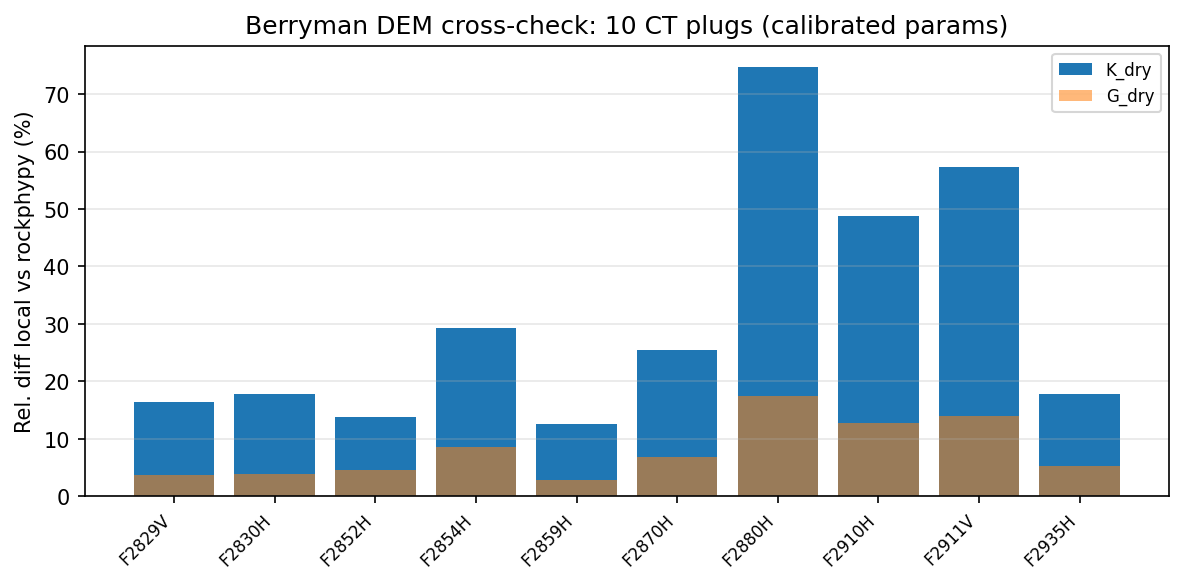
\includegraphics[width=0.82\linewidth]{figures/fig2_dem_rockphypy_crosscheck}
  \caption{Diferença relativa entre a implementação local e a
           biblioteca RockPhysicsPy (v0.0.2) em $K_{\mathrm{dry}}$ e
           $G_{\mathrm{dry}}$: dez plugs CT, parâmetros calibrados por HFU,
           junho de 2026.}
  \label{fig:dem_rockphypy_crosscheck}
\end{figure}

Na Figura~\ref{fig:dem_rockphypy_crosscheck}, as barras azuis ($K_{\mathrm{dry}}$)
dominam a divergência---coerente com o bulk ser o grau de liberdade mais
sensível à troca $K \leftrightarrow G$ na chamada de \emph{PQ}.
A ordem de grandeza (dezenas de por cento em $K_{\mathrm{dry}}$, unidades de
por cento a dezenas em $G_{\mathrm{dry}}$) descarta arredondamento ou
$\Delta y$ como explicação principal e reforça o diagnóstico de
erro na rotina diferencial publicada.

\section{Validação contra laboratório (ROCKPHYS)}
\label{sec:lab}

\subsection{Antes da calibração}

Com parâmetros apenas do microCT, o DEM superestima \Vp{} em relação ao
laboratório (Tabela~\ref{tab:lab_uncal}).
A Figura~\ref{fig:vp_lab_uncal} mostra pontos sistematicamente acima da linha
1:1, especialmente em amostras com \Vp{} laboratorial mais baixo.

\begin{table}[H]
  \centering
  \caption{Validação DEM vs laboratório (dez plugs CT, 22,1~MPa,
           eixo~$Z$, sem calibração).}
  \label{tab:lab_uncal}
  \begin{tabular}{lcc}
    \toprule
    Métrica & Valor & Unidade \\
    \midrule
    MAPE \Vp & 26,3 & \% \\
    RMSE \Vp & 1,37 & km/s \\
    Viés \Vp & $+1{,}22$ & km/s \\
    \Vp{} médio laboratório & 5,05 & km/s \\
    \Vp{} médio DEM & 6,27 & km/s \\
    \bottomrule
  \end{tabular}
\end{table}

Nessa linha de base, o viés de $+1{,}2$~km/s indica que o modelo a seco, com $\alpha$ do microCT,
trata a rocha como excessivamente rígida.
O MAPE de 26\% é inaceitável para uso interpretativo, mas cumpre o papel de
\emph{linha de base}: quantifica o quanto a calibração por HFU precisa
corrigir antes da extrapolação ao perfil.

\begin{figure}[H]
  \centering
  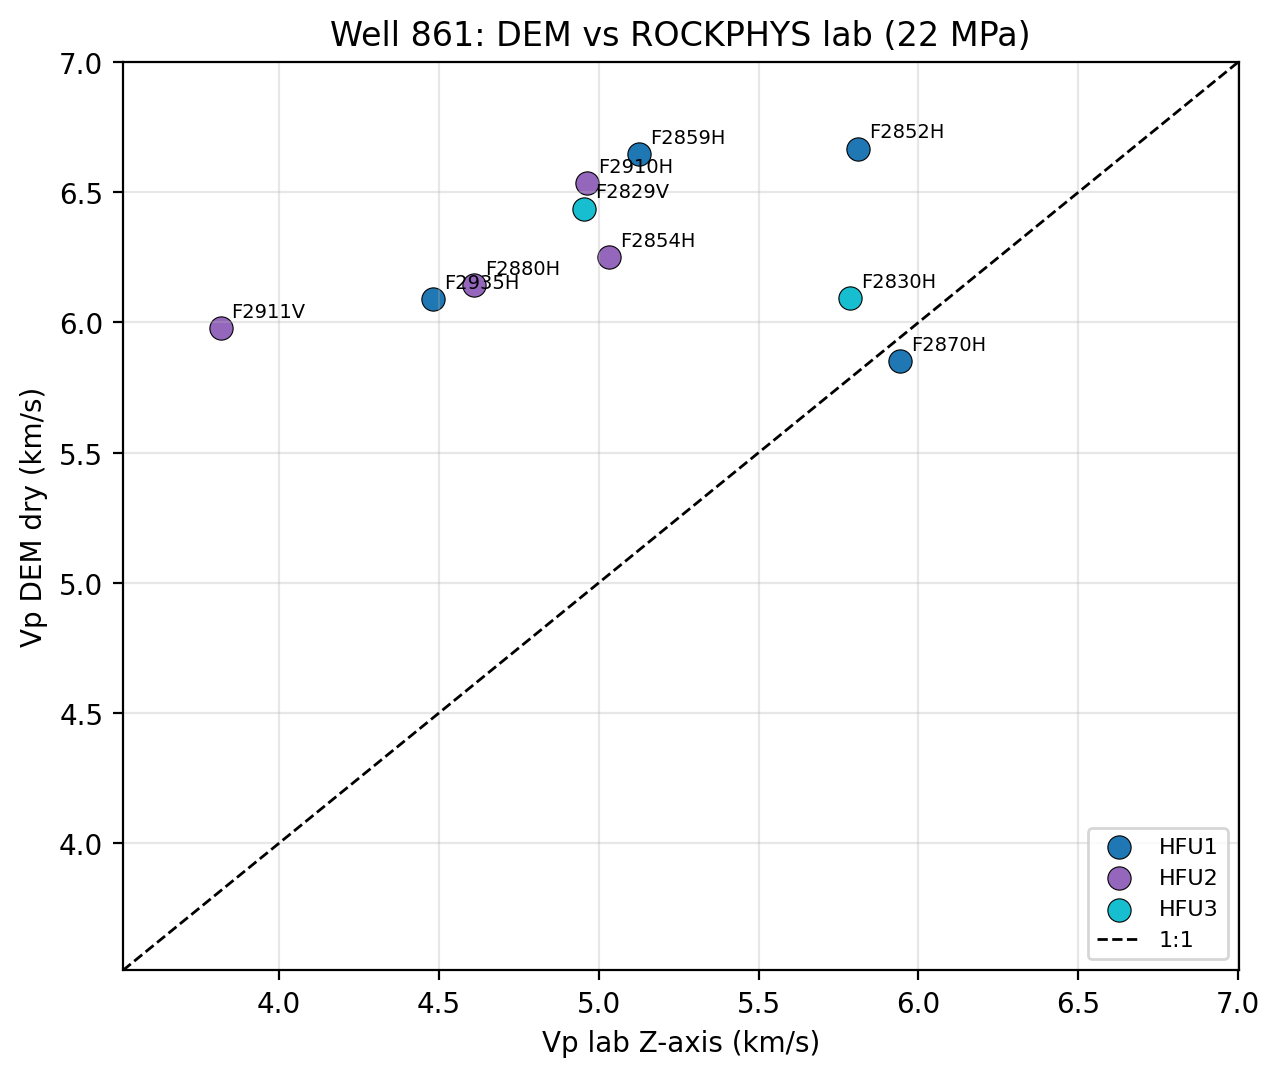
\includegraphics[width=0.78\linewidth]{figures/fig2_vp_dem_vs_lab}
  \caption{\Vp{} DEM versus \Vp{} de laboratório (eixo~$Z$, 22,1~MPa), antes
           da calibração por HFU. Pontos acima da diagonal indicam
           superestimação do modelo.}
  \label{fig:vp_lab_uncal}
\end{figure}

A Figura~\ref{fig:vp_lab_uncal} confirma visualmente que a maioria dos plugs cai acima da linha 1:1.
A dispersão por HFU sugere que um único $\alpha$ global não bastaria:
cada unidade de fluxo exige parâmetros distintos, justificando a calibração
segmentada adiante.

\subsection{Após calibração inversa}

A calibração por HFU reduz o MAPE \emph{in-sample} para $\approx 9\%$ e
praticamente elimina o viés (Tabela~\ref{tab:calib}).
A Tabela~\ref{tab:hfu_params} lista os parâmetros obtidos; a
Figura~\ref{fig:calib} mostra o ajuste plug a plug; a
Figura~\ref{fig:alpha} contrasta $\alpha$ calibrado com a mediana do microCT.

\begin{table}[H]
  \centering
  \caption{Parâmetros calibrados por HFU extrapolados ao perfil (configuração
           padrão, junho de 2026). $K_m$, $G_m$ e $\rho_m$ são os modulos da
           matriz após calibração; a Tabela~\ref{tab:app_hfu_matrix} detalha
           os valores CT e as escalas.}
  \label{tab:hfu_params}
  \small
  \begin{tabular}{ccccccccc}
    \toprule
    HFU & $n_{\mathrm{plugs}}$ &
    $\alpha_{\mathrm{calib}}$ & $\alpha_{\mathrm{CT}}$ &
    $K_m$ (GPa) & $G_m$ (GPa) & $\rho_m$ (g/cm$^3$) &
    Escala $K,G$ & Origem \\
    \midrule
    1 & 4 & 0,950 & 0,554 & 58,6 & 25,7 & 2,774 & 0,697 & laboratório \\
    2 & 4 & 0,182 & 0,554 & 59,0 & 25,8 & 2,766 & 0,709 & laboratório \\
    3 & 2 & 0,950 & 0,615 & 59,0 & 25,5 & 2,754 & 0,721 & laboratório \\
    4 & 0 & 0,566 & -- & 82,5 & 35,8 & 2,760 & 1,000 & \emph{fallback} \\
    \bottomrule
  \end{tabular}
\end{table}

Os parâmetros da Tabela~\ref{tab:hfu_params} mostram que, em HFU~1 e HFU~3, $\alpha$ calibrado saturou no teto (0,95), enquanto a
mediana microCT ficou em $\approx 0{,}55$--0,62---sinal de que a geometria
efetiva vista pela elástica de laboratório difere da morfologia local da
imagem CT.
A HFU~2 é a mais bem sustentada (quatro plugs, $\alpha$ calibrado 0,18).
A HFU~4 não tem suporte experimental: seus parâmetros são apenas uma
aproximação.
Com apenas dez plugs, a calibração é sensível a outliers: o plug
F2911V (laboratório F2911H, eixo~$Z$, 22,1~MPa) apresenta \Vp{} laboratorial
anormalmente baixa ($\approx 3{,}8$~km/s) e distorce o ajuste da HFU~2 na
configuração padrão.
O pipeline oferece modo \emph{robust} (exclusão de F2911V), com MAPE
\emph{in-sample} global caindo de 9,1\% para $\approx 7{,}5\%$ e o LOO de
14,8\% para $\approx 12{,}8\%$; a rodada de produção documentada aqui usa a
configuração padrão com dez plugs, salvo análise de sensibilidade explícita.
A calibração por HFU deve ser lida como \textbf{ajuste local ao poço~861},
não como prova de transferência interpoços.

\begin{table}[H]
  \centering
  \caption{Impacto da calibração inversa (dez plugs, ajuste
           \emph{in-sample}).}
  \label{tab:calib}
  \begin{tabular}{lccc}
    \toprule
    & MAPE (\%) & RMSE (km/s) & Viés (km/s) \\
    \midrule
    Antes & 26,3 & 1,37 & $+1{,}22$ \\
    Depois & 9,1 & 0,52 & $-0{,}01$ \\
    \bottomrule
  \end{tabular}
\end{table}

A Tabela~\ref{tab:calib} quantifica a queda de 26\% para 9\% no MAPE, confirmando que a calibração captura a
maior parte do desvio sistemático.
Porém, \emph{in-sample} o modelo foi ajustado nos mesmos pontos que avalia:
a Seção~\ref{sec:loo} testa se esse ajuste se mantém entre os dez plugs
quando um é excluído.

\begin{figure}[H]
  \centering
  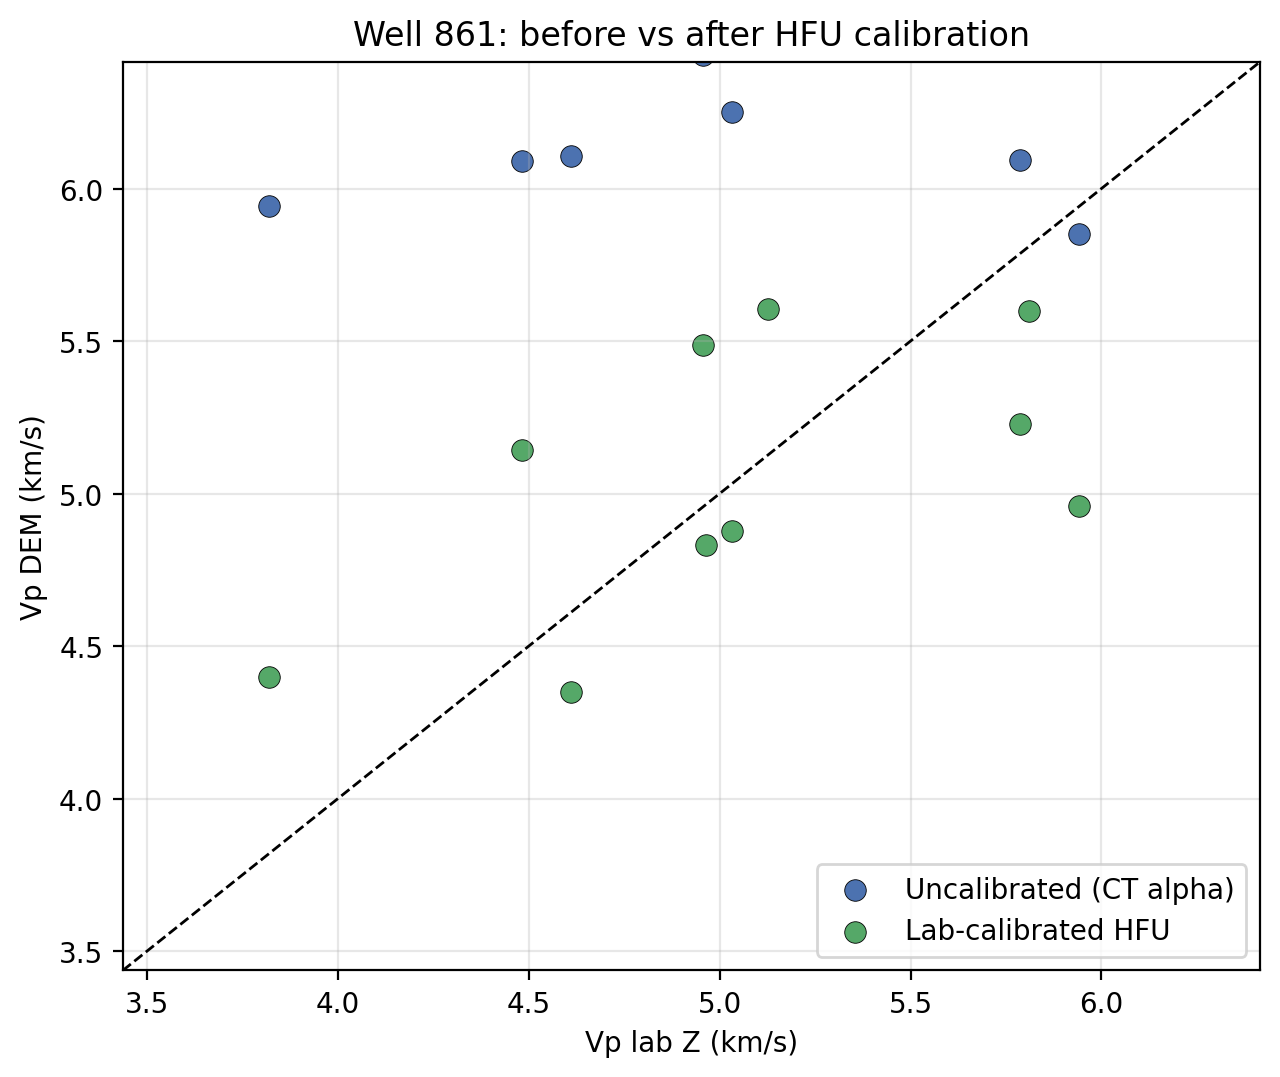
\includegraphics[width=0.82\linewidth]{figures/fig2_vp_calib_before_after}
  \caption{\Vp{} antes e depois da calibração por HFU nos plugs de
           laboratório. Após o ajuste, os pontos aproximam-se da linha 1:1.}
  \label{fig:calib}
\end{figure}

A Figura~\ref{fig:calib} mostra que cada plug aproxima-se da diagonal após o ajuste por HFU, confirmando que a
calibração cumpre seu objetivo \emph{in-sample}.
A dispersão residual antecipa o afastamento de cerca de seis pontos
percentuais no LOO (Tabela~\ref{tab:loo}).

\begin{figure}[H]
  \centering
  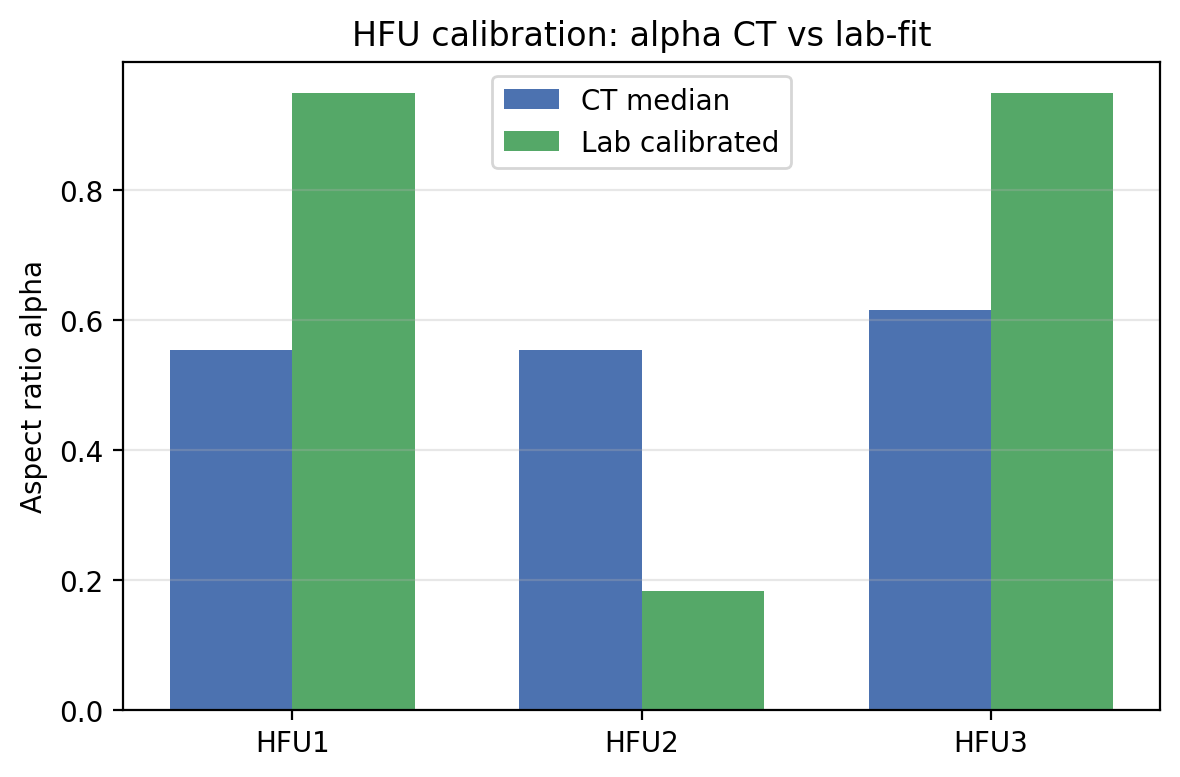
\includegraphics[width=0.72\linewidth]{figures/fig2_alpha_by_hfu}
  \caption{Razão de aspecto calibrada versus mediana do microCT por HFU.
           Barras divergentes indicam que a geometria CT, sozinha, não fecha
           o laboratório.}
  \label{fig:alpha}
\end{figure}

Por sua vez, a Figura~\ref{fig:alpha} contrasta $\alpha$ calibrado com a mediana do microCT: a HFU~2 é o caso em que a geometria CT e a calibração laboratorial
mais se aproximam ($\alpha$ calibrado 0,18 versus mediana CT $\approx 0{,}55$,
ainda distantes, porém com melhor fechamento elástico global).
Nas HFU~1 e~3, $\alpha$ calibrado satura no teto (0,95), sinal de limite do
modelo ou de poucos graus de liberdade com apenas dois a quatro plugs.

\subsection{Validação leave-one-plug-out (LOO)}
\label{sec:loo}

Para evitar otimismo da calibração \emph{in-sample}, repetimos o ajuste
excluindo um plug por vez (dez rodadas).
O MAPE LOO ficou em $\approx 14{,}8\%$, RMSE $\approx 0{,}85$~km/s e viés
$\approx -0{,}07$~km/s (Tabela~\ref{tab:loo}).

\begin{table}[H]
  \centering
  \caption{Validação LOO: calibração refeita a cada exclusão de um
           plug (dez folds).}
  \label{tab:loo}
  \begin{tabular}{lcc}
    \toprule
    Métrica & LOO & \emph{In-sample} \\
    \midrule
    MAPE \Vp (\%) & 14,8 & 9,1 \\
    RMSE \Vp (km/s) & 0,85 & 0,52 \\
    Viés \Vp (km/s) & $-0{,}07$ & $-0{,}01$ \\
    \bottomrule
  \end{tabular}
\end{table}

Comparando as colunas da Tabela~\ref{tab:loo}, o MAPE LOO ($\approx 15\%$) é cerca de seis pontos percentuais pior que o
\emph{in-sample}---diferença esperada e saudável.
O viés praticamente nulo no LOO indica que o modelo não está
sistematicamente alto ou baixo no laboratório quando um plug é excluído
entre os dez do poço~861---não implica extrapolação a outros poços.
Este patamar ($\approx 15\%$, RMSE $\approx 0{,}85$~km/s) é o limite superior
de erro esperado e serve de referência para julgar o confronto com o sónico
de perfil (Seção~\ref{sec:dlis}).
Convém antecipar que o LOO é a métrica mais severa do conjunto: com dez
plugs distribuídos em três HFU, retirar uma amostra remove entre 25\% e 50\%
do suporte experimental da sua unidade, o que penaliza mais do que a
extrapolação de perfil, onde os parâmetros usam todos os plugs disponíveis.

\subsection{Teste A/B: DEM multiescala sequencial}
\label{sec:multiscale_ab}

A referência interna do projeto (scripts Equinor em
\texttt{refs\_scripts\_dem\_multiscale}) modela meso-macroporos e
microporos como \textbf{inclusões DEM sequenciais}, com frações
\texttt{phi\_meso\_macropores\_vv} e \texttt{phi\_micropores\_vv} do
microCT e inversão unidimensional da razão de aspecto dos microporos
(\emph{grid search}, sem regressão global).
Antes de estender o perfil de 87 linhas, executamos um experimento
\textbf{aditivo} (fase~2f) que \textbf{não altera} a calibração monoescala
nem o pipeline de extrapolação documentado nas seções anteriores.

Comparamos três leituras nos dez plugs CT:
\begin{itemize}
  \item \textbf{M1} --- monoescala calibrado por HFU (baseline desta etapa);
  \item \textbf{M2a/M2b \emph{oracle}} --- multiescala com busca de
        $\alpha_{\mathrm{micro}}$ para fechar \Vp{} de laboratório no
        \emph{mesmo} plug (teto diagnostico, nao e previsao);
  \item \textbf{M2b \emph{forward}} --- medianas CT por HFU para fracoes e
        $\alpha_{\mathrm{meso}}$; mediana dos $\alpha_{\mathrm{micro}}$
        \emph{oracle} nos plugs de treino do HFU; previsao do plug alvo
        \textbf{sem} inverter $\alpha_{\mathrm{micro}}$ no plug avaliado
        (proxy honesto da extrapolacao ao perfil).
\end{itemize}

A escala $K_m$, $G_m$ herdada da calibracao M1 permanece fixa em todos os
cenarios multiescala; nao ha novo \texttt{scipy.optimize} por HFU
(cenario M2c, fora de escopo).

A Tabela~\ref{tab:multiscale_ab} resume as metricas principais.
O modo \emph{oracle} reduz o MAPE \emph{in-sample} para $\approx 3\%$,
mas isso reflete um parametro livre por plug ajustado ao alvo---nao
comparavel ao M1, que compartilha $\alpha$ entre plugs da mesma HFU.
No modo \emph{forward}, relevante para o perfil, o MAPE \emph{in-sample}
fica em $\approx 8{,}7\%$ contra $\approx 9{,}1\%$ do M1---ganho de apenas
$\approx 0{,}4$~p.p., com RMSE ligeiramente pior (0,54 contra 0,52~km/s).
No LOO \emph{forward}, o MAPE cai de $\approx 14{,}8\%$ (M1) para
$\approx 12{,}0\%$ (M2b)---ganho de $\approx 2{,}9$~p.p., porém
\textbf{sem} confirmacao \emph{in-sample}.
Adotamos o criterio pre-registrado: manter monoescala quando o ganho LOO
nao se acompanha de melhora \emph{in-sample} acima de 2~p.p.
\textbf{Conclusao:} nao ha evidencia suficiente para substituir o perfil
monoescala com $\alpha$ efetivo por HFU; as fracoes multiescala do CT
permanecem documentadas para uso futuro, mas nao entram no produto atual.

\begin{table}[H]
  \centering
  \caption{Teste A/B multiescala versus monoescala calibrado (dez plugs CT,
           junho de 2026). M2b \emph{forward}: medianas HFU, sem ajuste de
           $\alpha_{\mathrm{micro}}$ no plug avaliado.}
  \label{tab:multiscale_ab}
  \small
  \begin{tabular}{llcc}
    \toprule
    Modelo & Escopo & MAPE \Vp{} (\%) & RMSE (km/s) \\
    \midrule
    M1 monoescala calibrado & In-sample & 9,1 & 0,52 \\
    M2a multiescala \emph{oracle} & In-sample & 3,0 & 0,37 \\
    M2b multiescala \emph{forward} & In-sample & 8,7 & 0,54 \\
    M1 monoescala calibrado & LOO & 14,8 & 0,85 \\
    M2b multiescala \emph{forward} & LOO & 12,0 & 0,78 \\
    \bottomrule
  \end{tabular}
\end{table}

A Figura~\ref{fig:multiscale_ab_panel} contrasta M1 e M2b \emph{forward} no plano
1:1; o painel (b) mostra que o modo \emph{oracle} pode reduzir erro plug a
plug, mas o \emph{forward} acompanha o M1.

\begin{figure}[H]
  \centering
  \begin{subfigure}[t]{0.48\linewidth}
    \centering
    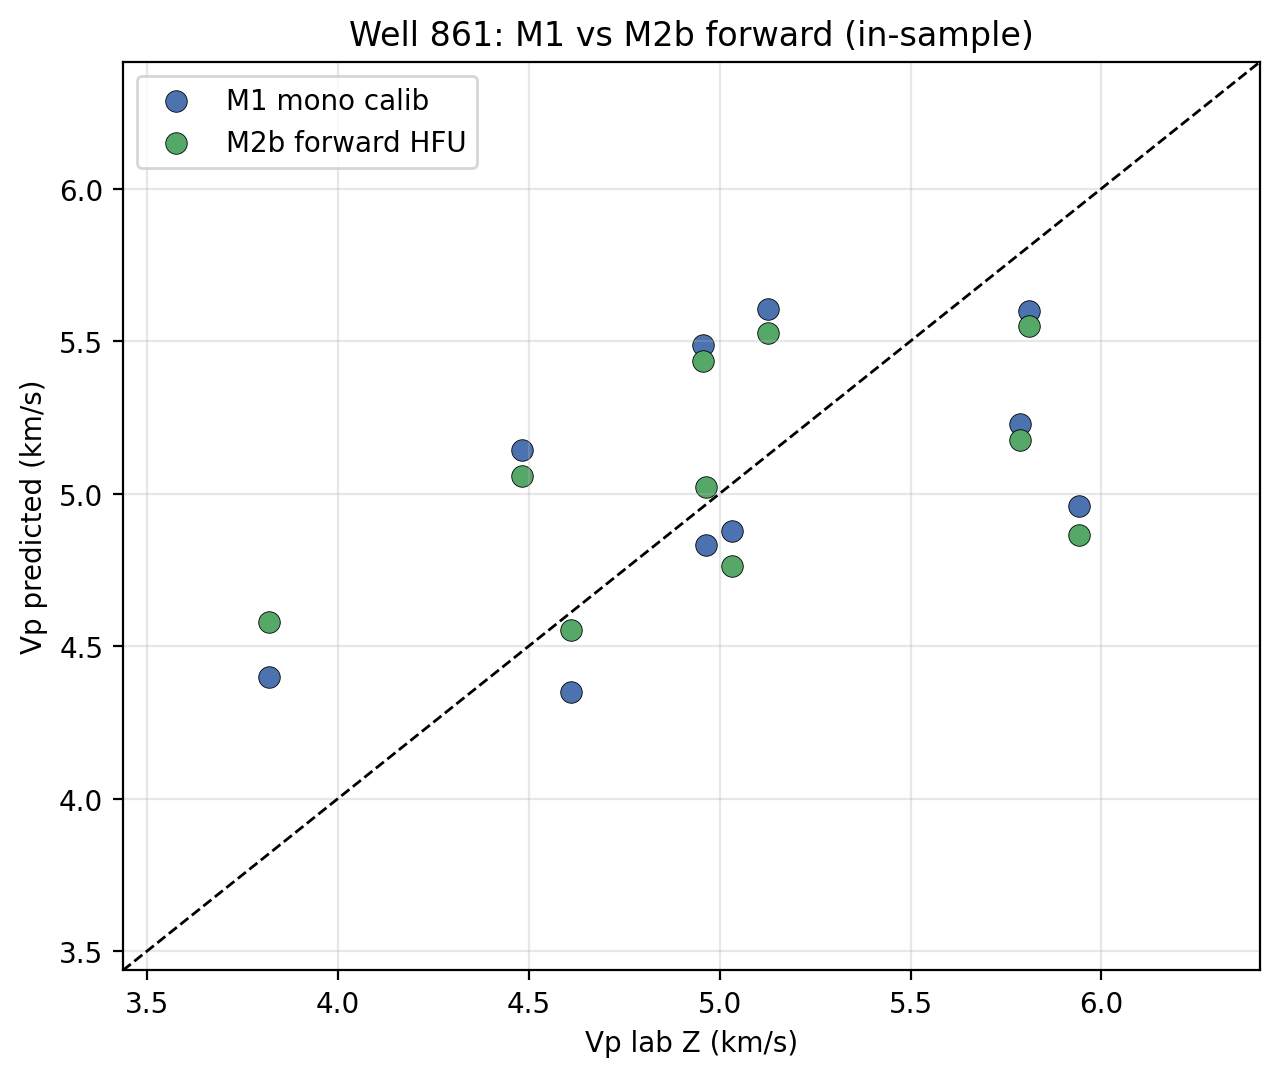
\includegraphics[width=\linewidth]{figures/fig2_multiscale_ab_crossplot}
    \caption{M1 vs M2b \emph{forward} (\emph{in-sample}).}
    \label{fig:multiscale_ab_crossplot}
  \end{subfigure}
  \hfill
  \begin{subfigure}[t]{0.48\linewidth}
    \centering
    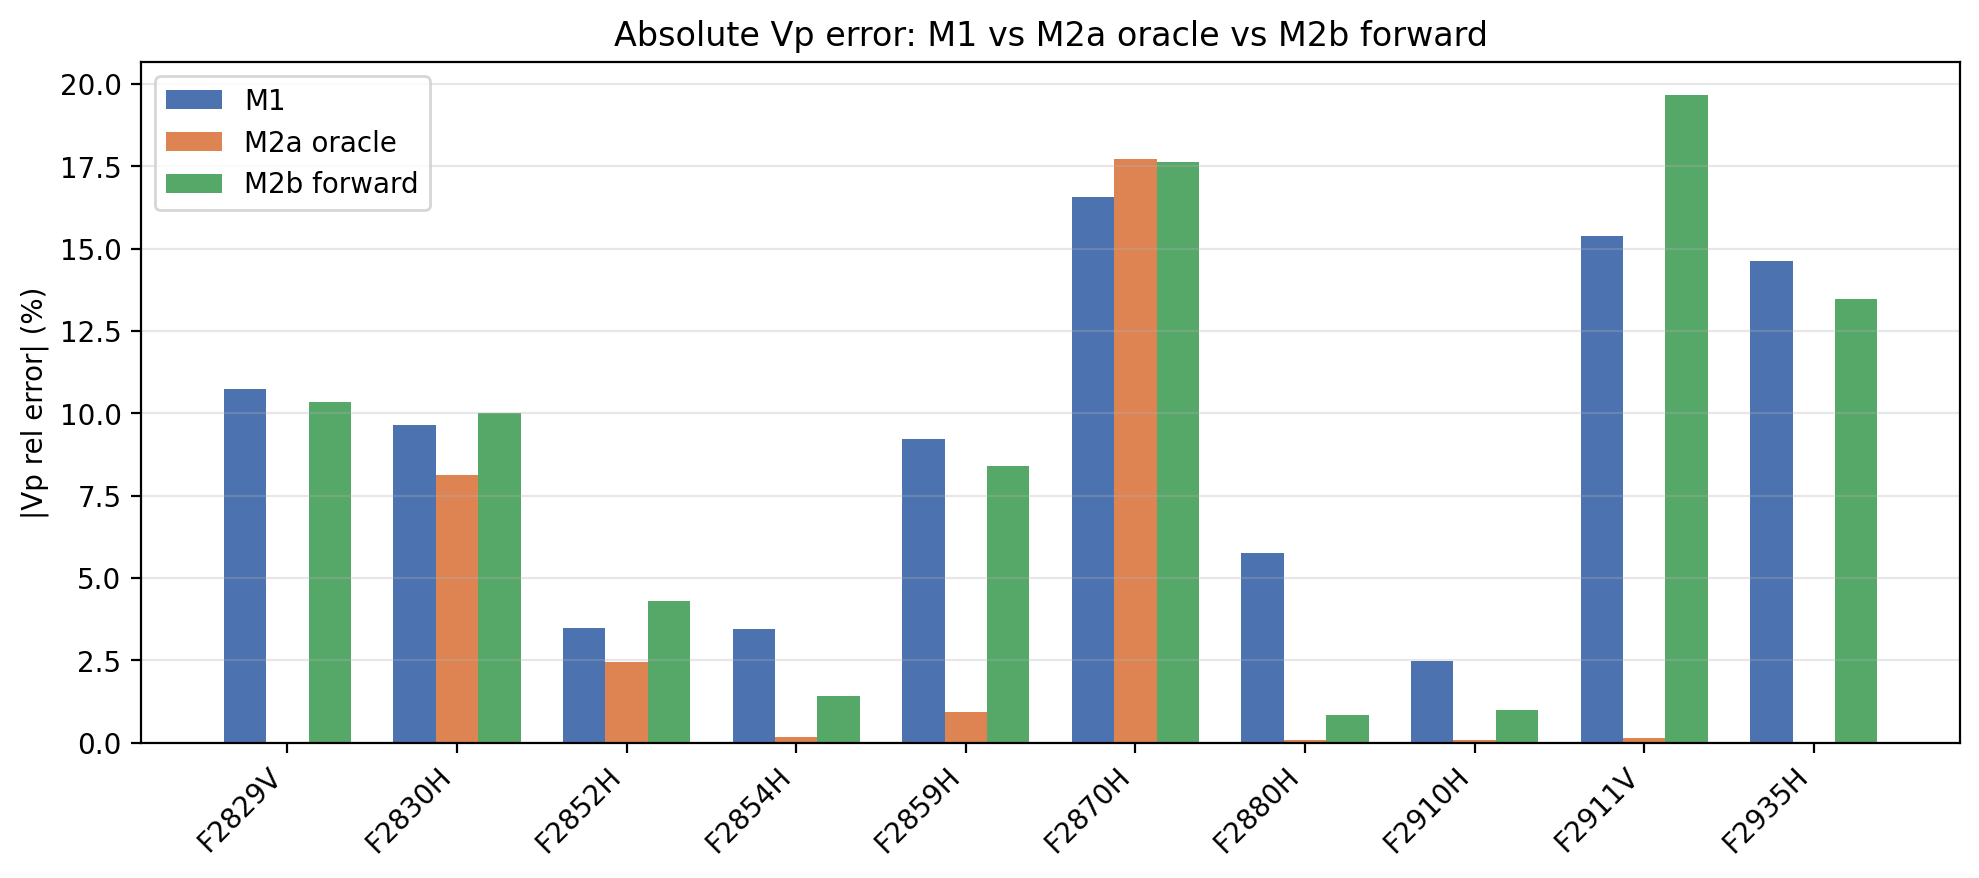
\includegraphics[width=\linewidth]{figures/fig2_multiscale_ab_error_by_plug}
    \caption{|Erro relativo| por plug: M1, M2a \emph{oracle}, M2b \emph{forward}.}
    \label{fig:multiscale_ab_err}
  \end{subfigure}
  \caption{Teste A/B multiescala (fase~2f): o modo \emph{forward} nao supera
           o monoescala calibrado de forma consistente.}
  \label{fig:multiscale_ab_panel}
\end{figure}

Sete dos dez plugs apresentam microporosidade CT inferior a 10\% do espaco
poroso; nesses casos a cadeia sequencial colapsa para uma unica inclusao
dominante.
No perfil de 87 linhas, as fracoes multiescala seriam, no melhor caso,
\textbf{constantes por HFU} (medianas de dois a quatro plugs)---a mesma
limitacao de homogeneidade intra-HFU do $\alpha$ unico ja discutida na
Seção~\ref{sec:profile}.
O experimento completo, scripts e \texttt{metrics.json} estao em
\texttt{dem\_sc\_runs/multiscale\_ab/}; o planejamento em
\texttt{planning/etapa2f\_dem\_multiscale\_ab\_poco861.md}.

\section{Extrapolação ao perfil completo (87 linhas)}
\label{sec:profile}

Com parâmetros calibrados, processamos as 87 linhas do perfil integrado.
\Vp{} médio $\approx 5{,}20$~km/s e \VpVs{} $\approx 1{,}82$
(Tabela~\ref{tab:profile}).
A entrada \phiND{} permanece alinhada à porosidade sónica do perfil
($r \approx 0{,}94$; Figura~\ref{fig:phi_sonic}).

\begin{table}[H]
  \centering
  \caption{Perfil calibrado (87 linhas, todas com status OK).}
  \label{tab:profile}
  \begin{tabular}{lcc}
    \toprule
    Grandeza & Valor & Unidade \\
    \midrule
    \Vp{} médio DEM & 5,20 & km/s \\
    \VpVs{} médio DEM & 1,82 & -- \\
    Pearson $r$ (\phiND{} vs \phiS) & 0,94 & -- \\
    Diferença relativa média DEM vs SC (\Vp) & 4,5 & \% \\
    \bottomrule
  \end{tabular}
\end{table}

Na Tabela~\ref{tab:profile}, o \Vp{} médio calibrado ($\approx 5{,}2$~km/s) aproxima-se do laboratório
($\approx 5{,}0$~km/s), coerente com o LOO.
A forte correlação \phiND{}--\phiS{} confirma que a porosidade de entrada
é confiável; isso não garante, por si só, que \Vp{} esteja correto---
apenas que a \emph{entrada} petrofísica está consistente com o sónico de
porosidade.

\begin{figure}[H]
  \centering
  \begin{subfigure}[t]{0.55\linewidth}
    \centering
    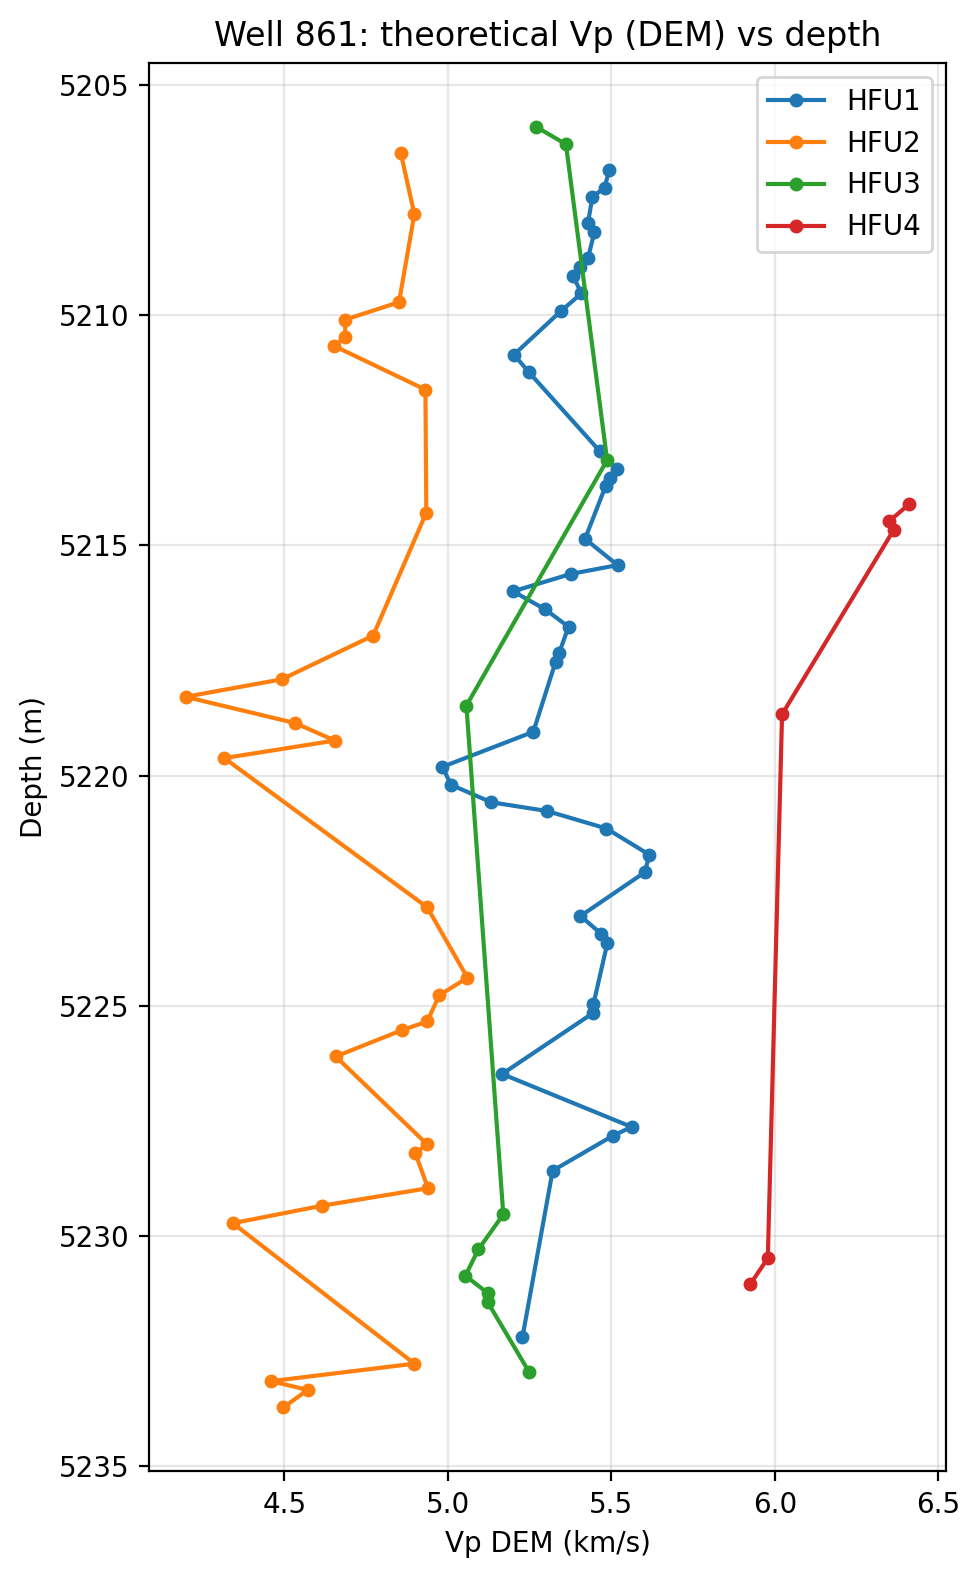
\includegraphics[width=\linewidth]{figures/fig2_vp_dem_depth}
    \caption{\Vp{} DEM versus profundidade por HFU.}
    \label{fig:vp_depth}
  \end{subfigure}
  \hfill
  \begin{subfigure}[t]{0.42\linewidth}
    \centering
    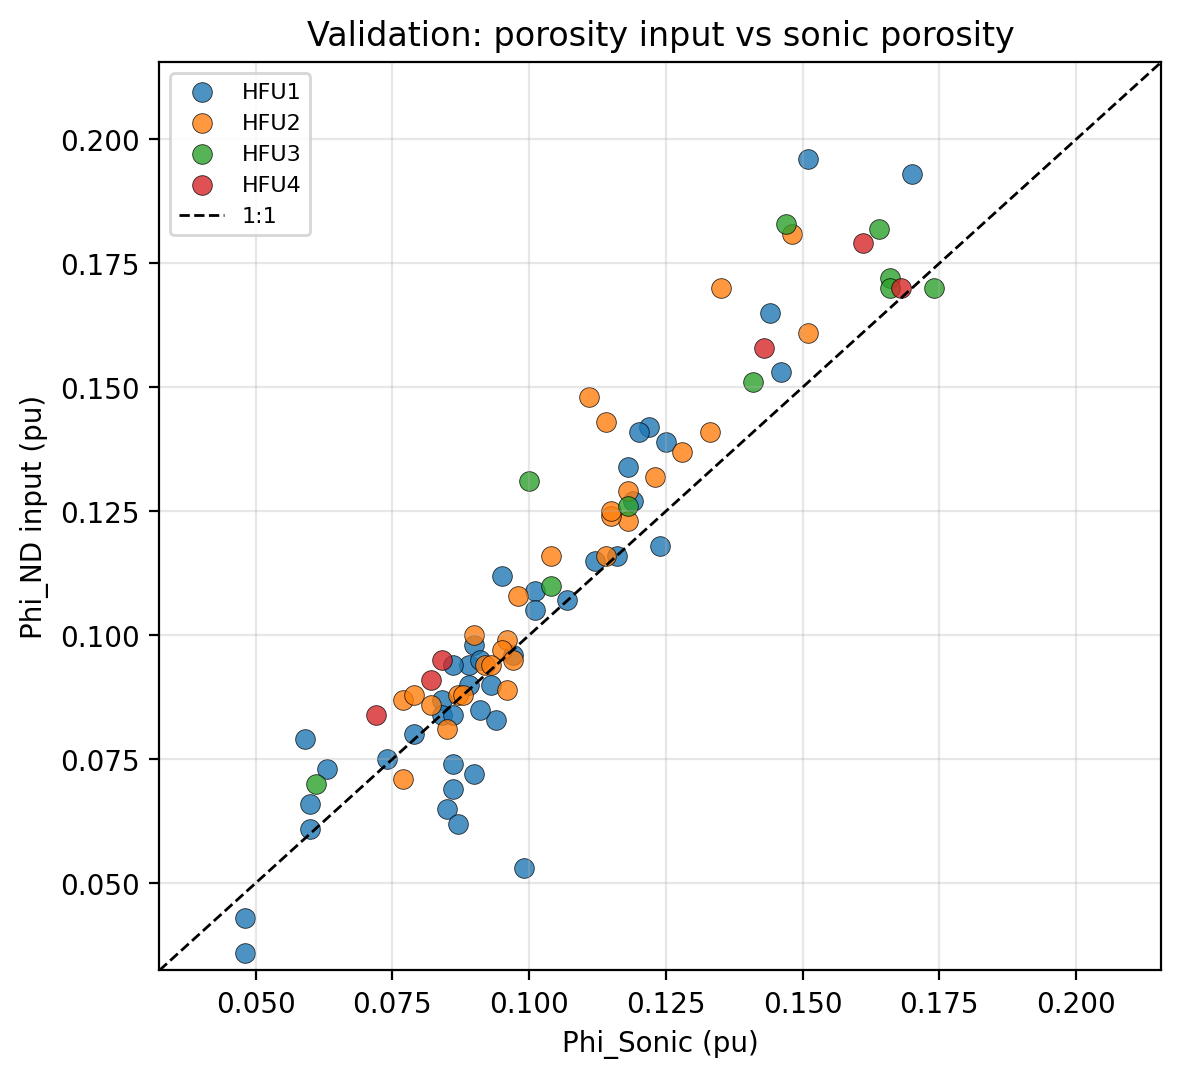
\includegraphics[width=\linewidth]{figures/fig2_phi_nd_vs_phi_sonic}
    \caption{\phiND{} versus \phiS{} (validação da entrada).}
    \label{fig:phi_nd_sonic}
  \end{subfigure}
  \caption{Perfil calibrado: saída elástica (a) e consistência de
           porosidade (b).}
  \label{fig:phi_sonic}
\end{figure}

A Figura~\ref{fig:phi_sonic} reúne dois painéis complementares.
\emph{Painel (a)---\Vp{} versus profundidade:}
As trilhas por HFU mostram a extrapolação ao longo do poço~861.
HFU~4 (seis pontos) tende a valores mais altos de \Vp{}, reflexo do
\emph{fallback} sem suporte de laboratório.

\emph{Painel (b)---\phiND{} versus \phiS:}
Os pontos agrupam-se próximos à diagonal 1:1, com $r \approx 0{,}94$.
Isso valida a escolha da Etapa~1 de usar \phiND{} como entrada conservadora
para a modelagem física.

\begin{figure}[H]
  \centering
  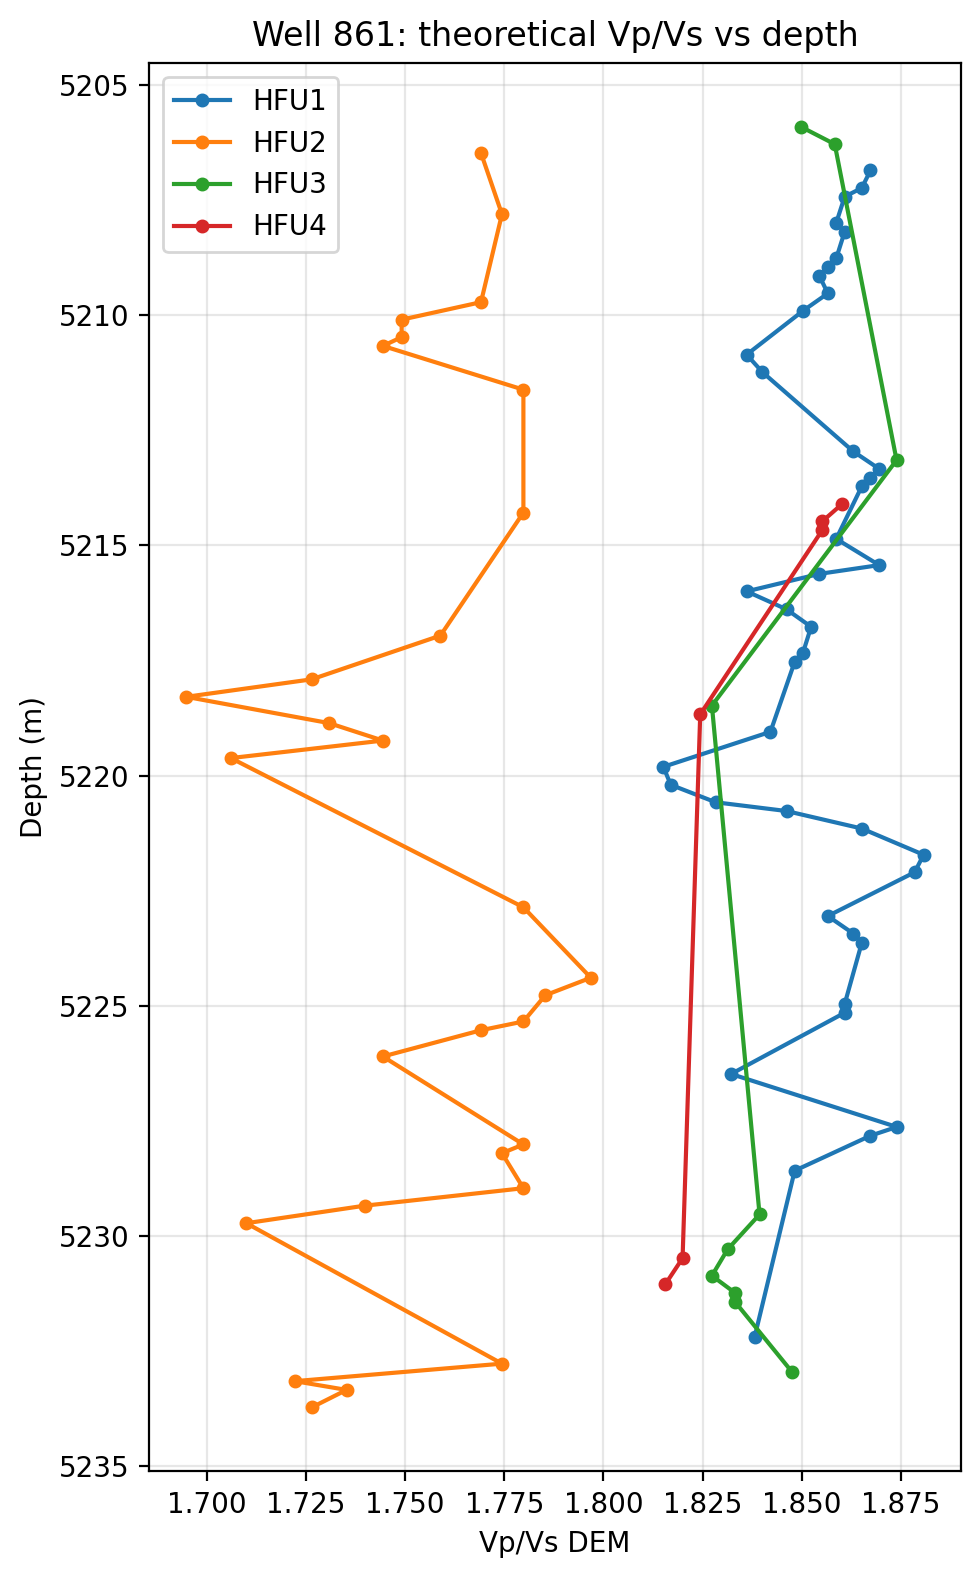
\includegraphics[width=0.55\linewidth]{figures/fig2_vpvs_depth}
  \caption{\VpVs{} DEM calibrado versus profundidade, colorido por HFU.}
  \label{fig:vpvs_profile}
\end{figure}

A Figura~\ref{fig:vpvs_profile} exibe a razão \VpVs{} ao longo do intervalo, variando modestamente entre 1,7 e 1,9---
faixa compatível com carbonatos e com o sónico de perfil analisado adiante.
A estabilidade de \VpVs{} é um resultado positivo: mesmo quando \Vp{}
absoluto desvia, a \emph{forma} elástica compressional/cisalhante pode
permanecer interpretável.

\section{Validação com perfil sónico (DLIS)}
\label{sec:dlis}

\subsection{Procedimento e cobertura}

Extraímos DTCO e DTSM do arquivo DSI, convertemos para \Vp{} e \Vs{} e
casamos cada uma das 87 profundidades do perfil DEM com a amostra sónica
mais próxima (tolerância 0,25~m).
O casamento foi completo: 87/87 linhas.

\subsection{Resultados globais}

Como resumido na Tabela~\ref{tab:dlis_global} e na linha ``Perfil sónico DSI''
da Tabela~\ref{tab:validation_summary}, o MAPE de \Vp{} ($\approx 9\%$) fica
abaixo do LOO laboratorial (Tabela~\ref{tab:loo}), mas o viés é
positivo ($+0{,}30$~km/s): o DEM calibrado a seco fica mais rápido que o
sónico \emph{in-situ}.
\VpVs{} apresenta acordo comparável na mesma tabela (erro médio absoluto
$\approx 0{,}07$; médias 1,77 versus 1,82).
A Figura~\ref{fig:dlis_vp} ilustra o confronto em profundidade e no plano 1:1;
a Figura~\ref{fig:dlis_vpvs} complementa com \VpVs{} e mapa de erro.

\begin{table}[H]
  \centering
  \caption{Validação do perfil DEM calibrado contra sónico DSI
           (87 linhas).}
  \label{tab:dlis_global}
  \begin{tabular}{lcc}
    \toprule
    Métrica & Valor & Unidade \\
    \midrule
    Profundidades casadas & 87/87 & -- \\
    MAPE \Vp & 8,7 & \% \\
    RMSE \Vp & 0,54 & km/s \\
    Viés \Vp (DEM $-$ sónico) & $+0{,}30$ & km/s \\
    Pearson $r$ (\Vp{} DEM vs sónico) & 0,34 & -- \\
    \Vp{} médio sónico & 4,90 & km/s \\
    \Vp{} médio DEM & 5,20 & km/s \\
    Erro médio absoluto \VpVs & 0,07 & -- \\
    \bottomrule
  \end{tabular}
\end{table}

Os numeros da Tabela~\ref{tab:dlis_global} pedem duas leituras.
O MAPE de $\approx 9\%$ situa-se abaixo do LOO laboratorial, mas isso
\textbf{não} significa que a extrapolação seja mais confiável que o
laboratório: o LOO é uma métrica deliberadamente severa (Seção~\ref{sec:loo}),
enquanto no perfil os parâmetros usam todos os plugs da HFU.
Mais informativo é o viés de $+0{,}30$~km/s, que responde por cerca de três
quartos do erro médio absoluto: o DEM superestima \Vp{} de forma consistente
frente ao sónico saturado.
Isso é fisicamente plausível: calibramos em plugs secos a 22,1~MPa e
aplicamos ao perfil sem correção de fluido, motivando a fase~2b
(Seção~\ref{sec:gassmann}).
A correlação positiva porém modesta ($r \approx 0{,}34$) mostra que o modelo
acompanha apenas parcialmente a variabilidade fina do sónico---esperado,
já que a única grandeza que varia ponto a ponto na cadeia é \phiND{}, com
$\alpha$ e a matriz fixos por HFU.

\subsection{Desempenho por HFU}

A Tabela~\ref{tab:dlis_hfu} detalha o erro por unidade de fluxo.

\begin{table}[H]
  \centering
  \caption{Erro de \Vp{} versus sónico de perfil, por HFU.}
  \label{tab:dlis_hfu}
  \begin{tabular}{ccccc}
    \toprule
    HFU & $n$ & \Vp{} sónico médio & \Vp{} DEM médio & MAPE (\%) \\
    \midrule
    1 & 42 & 5,00 & 5,38 & 8,0 \\
    2 & 29 & 4,88 & 4,72 & 3,3 \\
    3 & 10 & 4,61 & 5,22 & 13,6 \\
    4 & 6  & 4,77 & 6,18 & 30,4 \\
    \bottomrule
  \end{tabular}
\end{table}

Na Tabela~\ref{tab:dlis_hfu}, a HFU~2 ($\approx 3\%$) atinge o patamar
desejável para interpretação quantitativa---coerente com quatro plugs de
calibração e com o único viés negativo do conjunto ($-0{,}16$~km/s).
A HFU~1 cobre quase metade do perfil (42 linhas) com MAPE $\approx 8\%$:
utilizável, ainda que com viés positivo de $+0{,}38$~km/s.
A HFU~3 ($\approx 14\%$, dois plugs) e sobretudo a HFU~4 ($\approx 30\%$,
nenhum plug) indicam que os maiores erros se concentram nas unidades com
menor ou nenhum suporte experimental; a HFU~4 não deve entrar em produto
final sem novos dados.
O contraste é o achado central desta seção: o erro de perfil não é uma
propriedade uniforme do modelo, e sim uma função da unidade avaliada.
O número de plugs, isoladamente, não explica toda a variação---HFU~1 e
HFU~2 têm quatro plugs cada e diferem por um fator de 2,4 no MAPE
(8,0\% contra 3,3\%).
A Seção~\ref{sec:hfu_cautela} retoma esse ponto e discute o segundo fator
associado ao contraste, a saturação de $\alpha$ no teto do intervalo de
calibração.

\begin{figure}[H]
  \centering
  \begin{subfigure}[t]{0.48\linewidth}
    \centering
    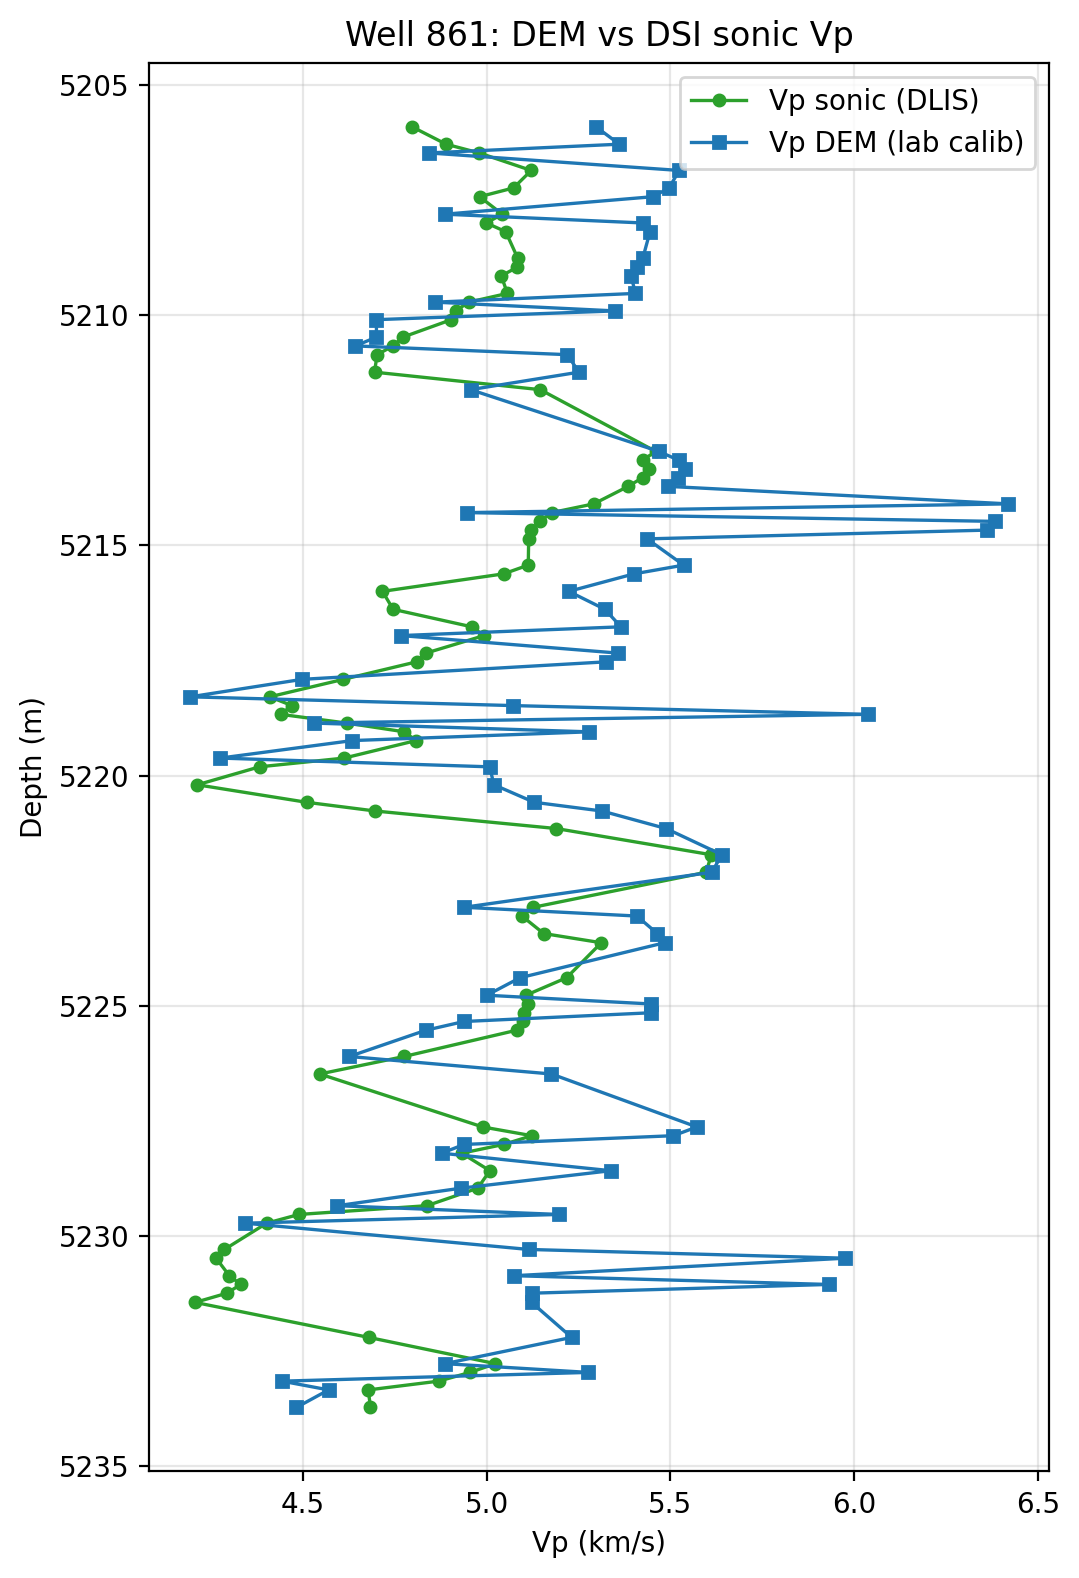
\includegraphics[width=\linewidth]{figures/fig2_vp_dem_vs_sonic_depth}
    \caption{Trilha de profundidade.}
    \label{fig:dlis_depth}
  \end{subfigure}
  \hfill
  \begin{subfigure}[t]{0.48\linewidth}
    \centering
    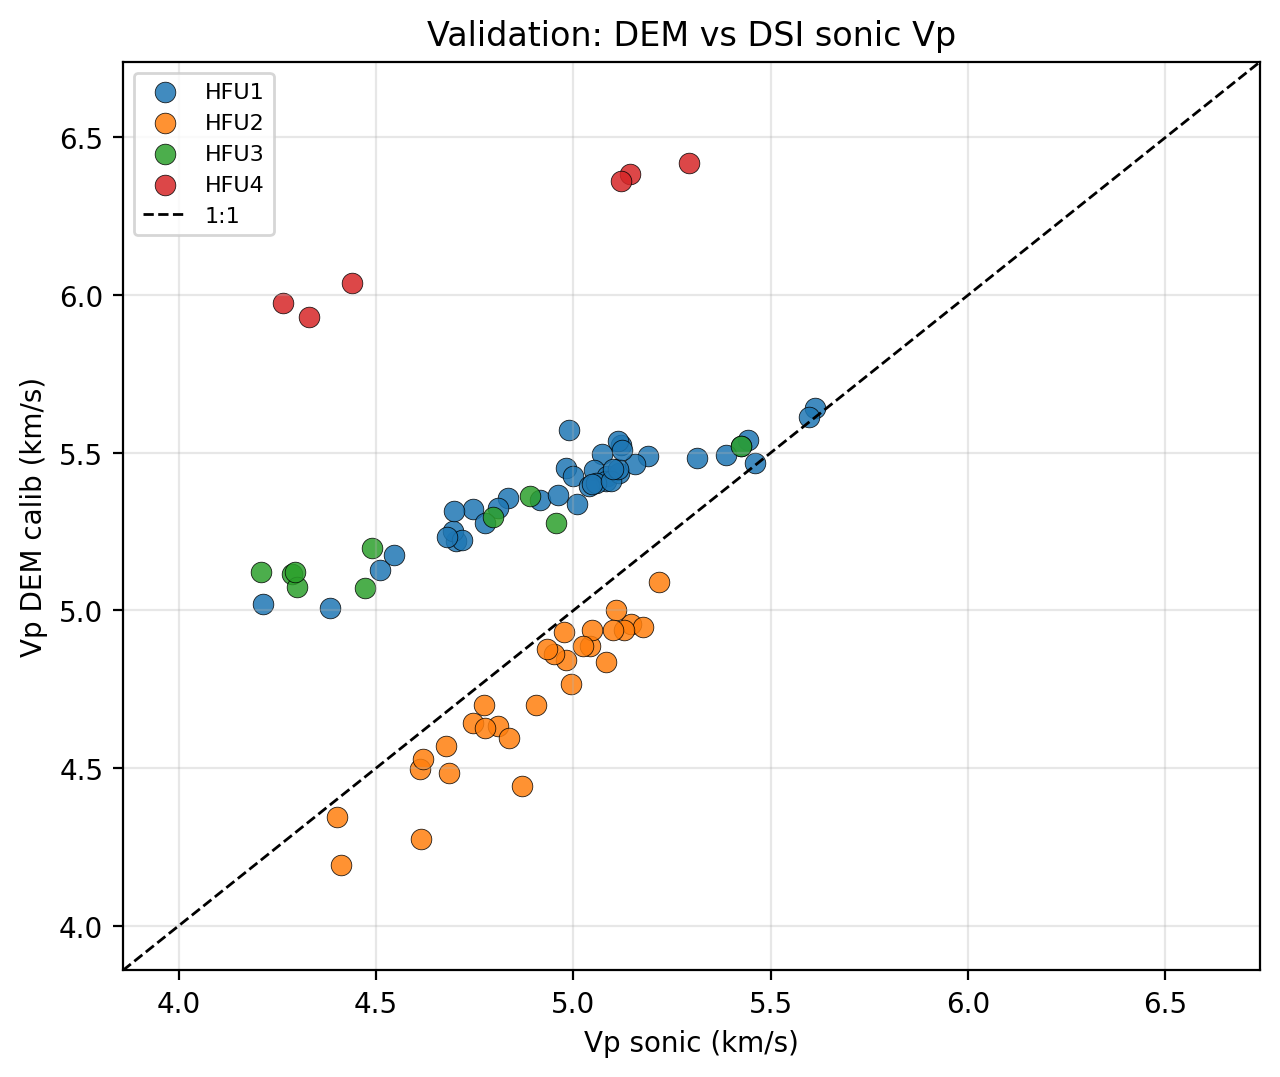
\includegraphics[width=\linewidth]{figures/fig2_vp_dem_vs_sonic_scatter}
    \caption{Dispersograma 1:1 por HFU.}
    \label{fig:dlis_scatter}
  \end{subfigure}
  \caption{Confronto \Vp{} DEM calibrado versus sónico DSI.}
  \label{fig:dlis_vp}
\end{figure}

A Figura~\ref{fig:dlis_vp} compara o confronto em dois painéis.
\emph{Painel (a)---trilha de profundidade:}
As duas curvas permanecem na mesma faixa de km/s ao longo de todo o
intervalo e compartilham as tendências de maior escala.
O DEM (azul) oscila mais que o sónico (verde) porque a troca de HFU muda
abruptamente $\alpha$ e a matriz entre linhas vizinhas: as excursões para
6~km/s e acima correspondem, sem exceção, às seis linhas de HFU~4.

\emph{Painel (b)---dispersograma:}
A HFU~2 concentra-se logo abaixo da diagonal (única unidade com viés
negativo) e a HFU~1 forma uma nuvem compacta pouco acima dela; a HFU~4
destaca-se isolada no topo, com superestimação de mais de 1~km/s.

\begin{figure}[H]
  \centering
  \begin{subfigure}[t]{0.48\linewidth}
    \centering
    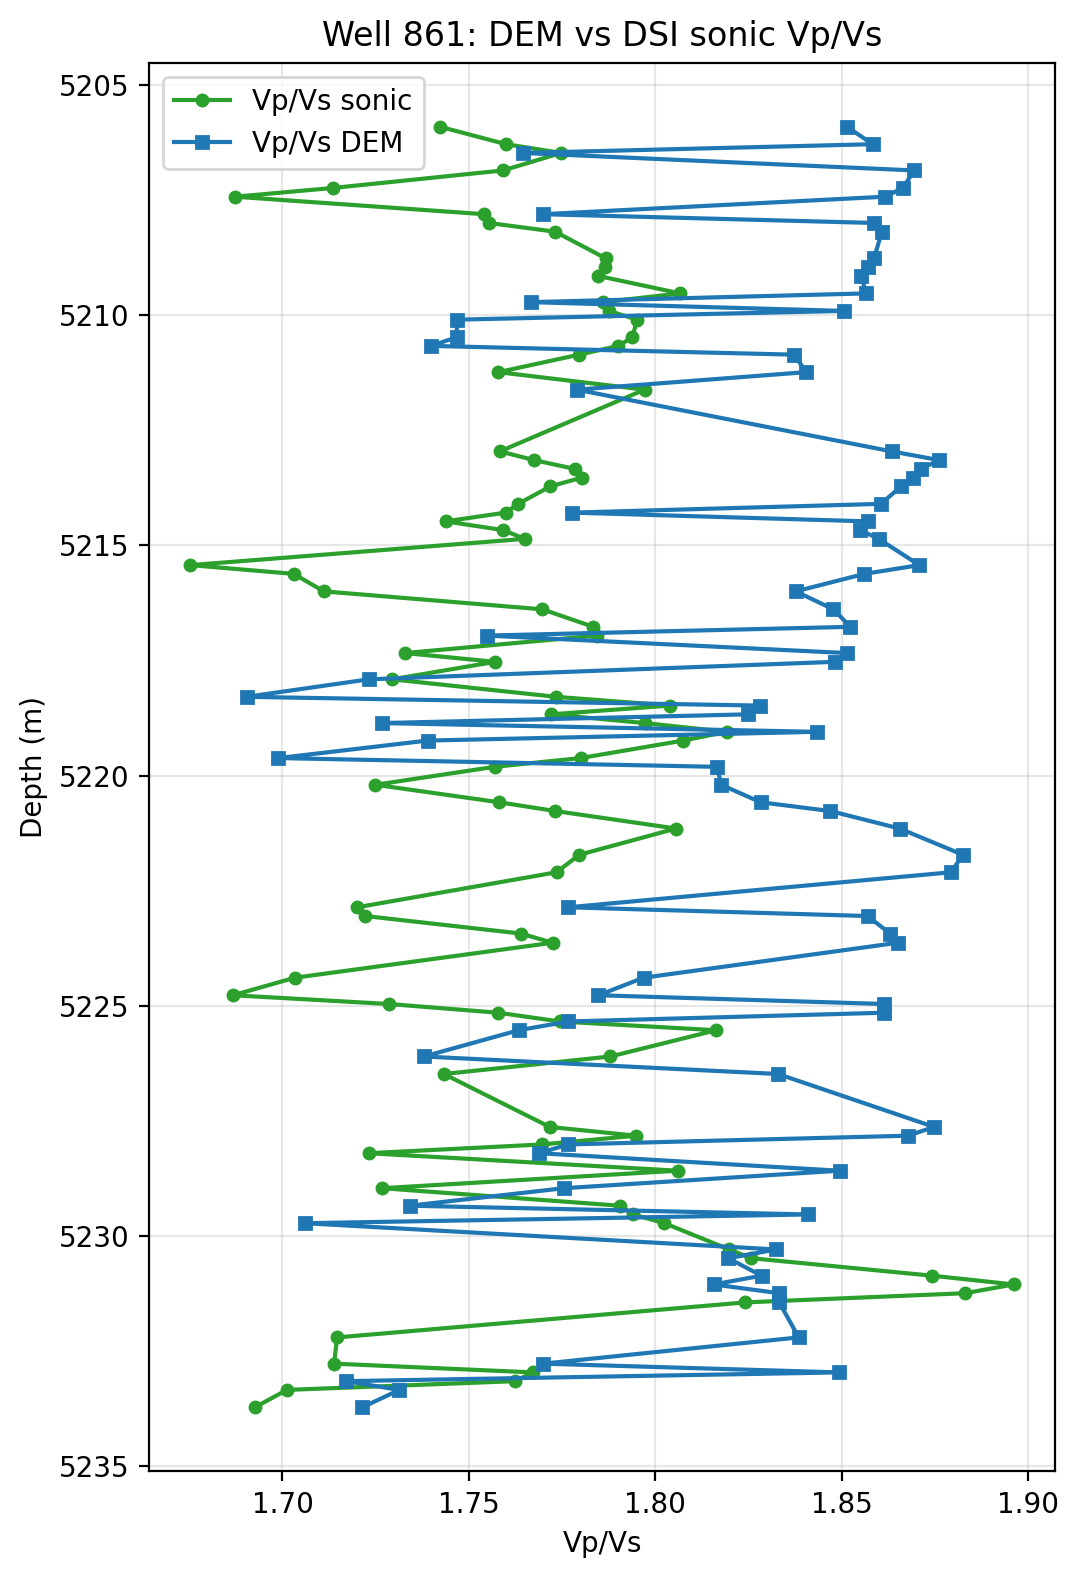
\includegraphics[width=\linewidth]{figures/fig2_vpvs_dem_vs_sonic}
    \caption{\VpVs{} sónico vs DEM.}
    \label{fig:dlis_vpvs_panel}
  \end{subfigure}
  \hfill
  \begin{subfigure}[t]{0.48\linewidth}
    \centering
    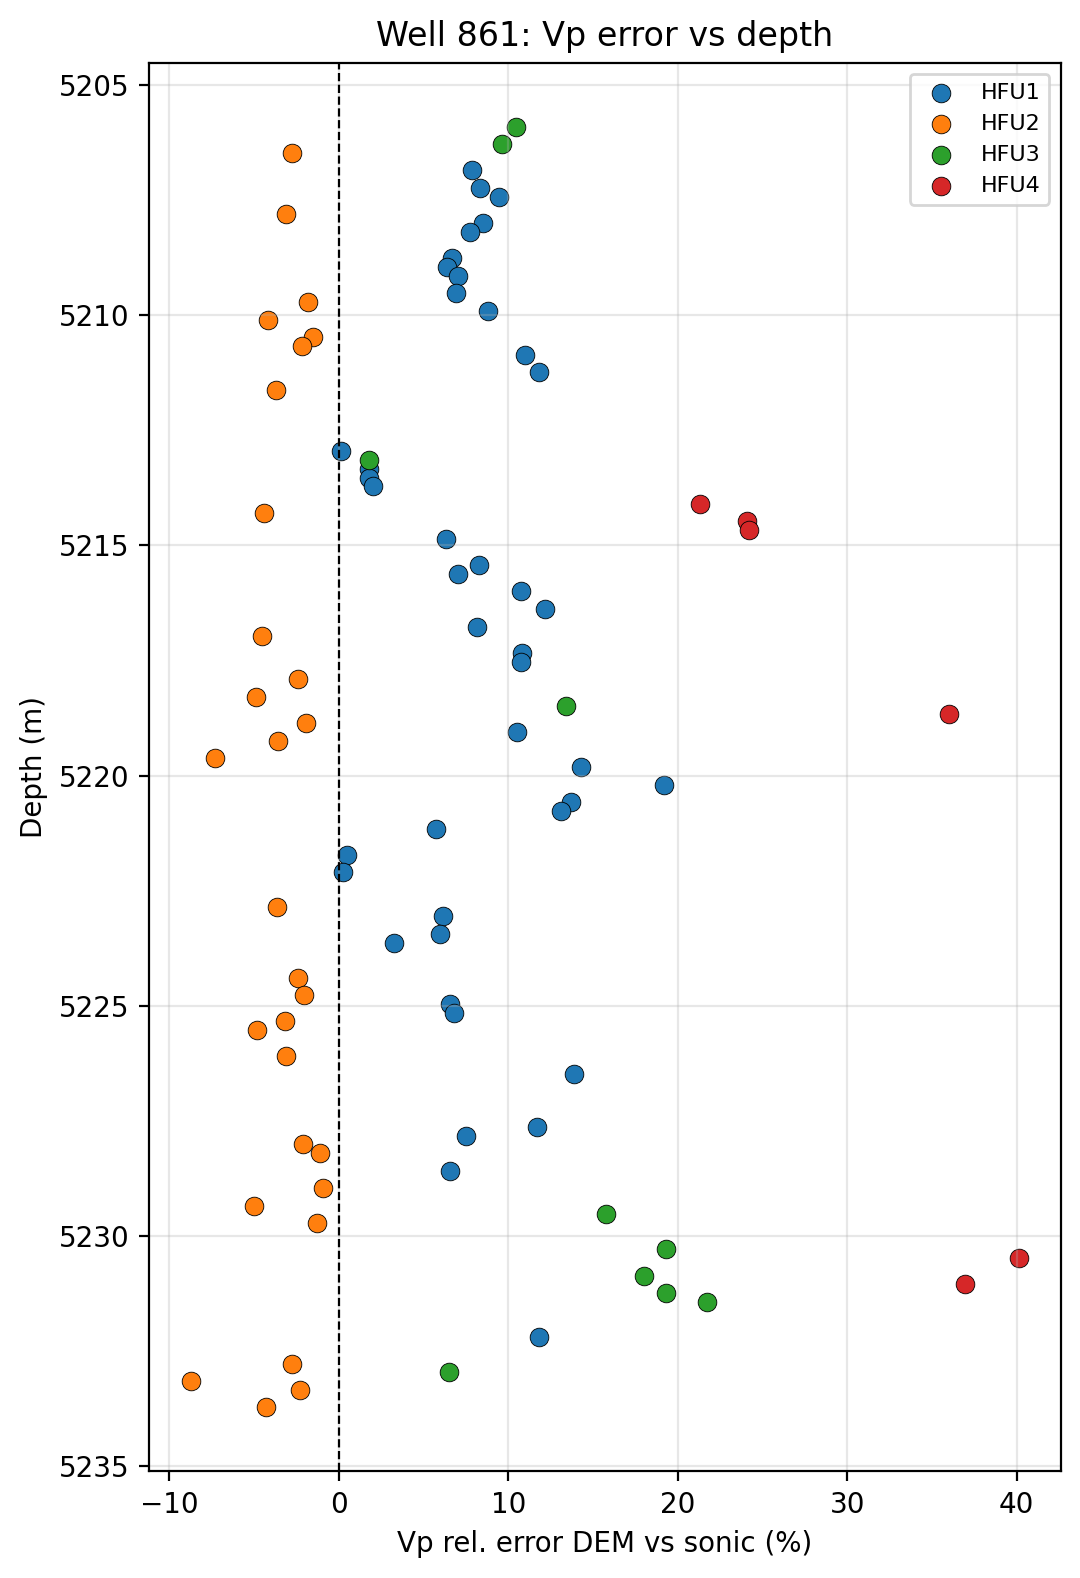
\includegraphics[width=\linewidth]{figures/fig2_vp_error_vs_depth}
    \caption{Erro relativo de \Vp{} vs profundidade.}
    \label{fig:dlis_error}
  \end{subfigure}
  \caption{Validação complementar: razão \VpVs{} e erro percentual.}
  \label{fig:dlis_vpvs}
\end{figure}

Na Figura~\ref{fig:dlis_vpvs}, o painel de \VpVs{} mostra trilhas próximas e
com amplitudes semelhantes (1,70--1,90), ainda que o DEM fique
sistematicamente cerca de 0,05 acima do sónico---a razão elástica é
capturada em forma, com pequeno deslocamento de nível.
O mapa de erro versus profundidade mostra que os desvios se organizam por
unidade de fluxo, não por profundidade: a HFU~2 ocupa a faixa
$-9\%$ a $+1\%$, a HFU~1 agrupa-se entre $+2\%$ e $+14\%$, a HFU~3 chega a
$+19\%$ e as seis linhas de HFU~4 aparecem isoladas entre $+21\%$ e $+40\%$.
A ausência de tendência com a profundidade descarta erro residual de
alinhamento e orienta onde a fase~2b (saturação) ou novos dados de
laboratório teriam maior impacto.

\subsection{Síntese das validações de \Vp{}}

A Tabela~\ref{tab:validation_summary} reúne, em um unico lugar, as métricas
de \Vp{} nas quatro escalas discutidas nas Seções~\ref{sec:lab}--\ref{sec:dlis}.
Ela deve ser lida junto com a Tabela~\ref{tab:validation_scales}: aquela
define \emph{o que} perguntamos; esta mostra \emph{quanto} erramos.

\begin{table}[H]
  \centering
  \caption{Síntese de validação de \Vp{} (km/s e \%), por escala.
           Rodada de producao: junho de 2026.}
  \label{tab:validation_summary}
  \small
  \begin{tabular}{lcccc}
    \toprule
    Escala & MAPE (\%) & RMSE (km/s) & Viés (km/s) & $n$ \\
    \midrule
    Lab, sem calibração & 26,3 & 1,37 & $+1{,}22$ & 10 \\
    Lab, in-sample & 9,1 & 0,52 & $-0{,}01$ & 10 \\
    Lab, LOO & 14,8 & 0,85 & $-0{,}07$ & 10 \\
    Perfil sónico DSI (seco) & 8,7 & 0,54 & $+0{,}30$ & 87 \\
    Perfil sónico DSI (Gassmann) & 7,3 & 0,48 & $+0{,}27$ & 87 \\
    Perfil DSI (Gassmann + NMR M3) & 8,5 & 0,47 & $+0{,}04$ & 87 \\
    \bottomrule
  \end{tabular}
\end{table}

A leitura conjunta da Tabela~\ref{tab:validation_summary} revela dois regimes
distintos de erro.
Nos plugs, o LOO ($\approx 15\%$) tem viés praticamente nulo: o erro é
dispersão, não deslocamento sistemático---o modelo acerta a média e erra a
amostra individual, sintoma de dez pontos sustentando três conjuntos de
parâmetros.
No perfil, o MAPE é menor ($\approx 9\%$ a seco, $\approx 7\%$ após
Gassmann), mas o viés é positivo e domina o erro.
São falhas de natureza oposta e a segunda é a mais tratável: um desvio
direcional pode ser modelado, ao passo que dispersão por falta de suporte
experimental só se resolve com mais plugs.
A linha Gassmann mostra redução modesta do viés
($+0{,}30 \rightarrow +0{,}27$~km/s), confirmando que a diferença
seca/saturada explica \emph{parte}, mas não a totalidade, do desvio contra o
DSI (Seção~\ref{sec:gassmann}).
A linha M3 (NMR multiescala) praticamente anula o viés ($+0{,}04$~km/s), mas
ao custo de MAPE maior, ficando fora do critério pre-registrado
(Seção~\ref{sec:multiscale_nmr}).

\section{Correção de saturação por Gassmann (fase~2b)}
\label{sec:gassmann}

\subsection{Fluido e equação}

Aplicamos substituição de fluido de Gassmann sobre o arcabouço seco
já calibrado por HFU, usando módulo de bulk do fluido $K_f \approx 2{,}2$~GPa
(água/salmoura de formação, default documentado na Tabela~\ref{tab:app_pvt}) e saturação total
($S_w = 1$).
A densidade saturada segue $\rho_{\mathrm{eff}} = (1-\phi)\rho_m + \phi\rho_f$.
O módulo de cisalhamento permanece $G_{\mathrm{sat}} \approx G_{\mathrm{dry}}$.
A relação de Gassmann (forma de Mavko) é:
\begin{equation}
  \label{eq:gassmann}
  K_{\mathrm{sat}} = K_{\mathrm{dry}}
    + \frac{\left(1 - K_{\mathrm{dry}}/K_0\right)^2}
           {\phi/K_f + (1-\phi)/K_0 - K_{\mathrm{dry}}/K_0^2},
\end{equation}
onde $K_0$ é o bulk mineral da matriz (aqui $K_m$ calibrado por HFU).
As velocidades saturadas usam $K_{\mathrm{sat}}$, $G_{\mathrm{sat}}$ e
$\rho_{\mathrm{eff}}$ na Equação~\eqref{eq:velocidades}.

\subsection{Resultados frente ao sónico}

A Tabela~\ref{tab:gassmann_compare} resume o efeito de Gassmann sobre as
métricas globais contra o DSI.
O \Vp{} médio cai de 5,20 para 5,17~km/s; o viés positivo diminui, mas
permanece material ($+0{,}27$~km/s).
A Figura~\ref{fig:gassmann_depth} confronta as três trilhas (sónico, DEM
seco e DEM saturado).

\begin{table}[H]
  \centering
  \caption{Comparacao global: perfil DEM seco versus Gassmann versus DSI
           (87 linhas, junho de 2026).}
  \label{tab:gassmann_compare}
  \begin{tabular}{lccc}
    \toprule
    Condicao & MAPE (\%) & RMSE (km/s) & Viés (km/s) \\
    \midrule
    DEM seco & 8,7 & 0,54 & $+0{,}30$ \\
    DEM + Gassmann & 7,3 & 0,48 & $+0{,}27$ \\
    \Vp{} médio DEM seco & -- & 5,20 & -- \\
    \Vp{} médio DEM Gassmann & -- & 5,17 & -- \\
    \Vp{} médio sónico & -- & 4,90 & -- \\
    \bottomrule
  \end{tabular}
\end{table}

\begin{figure}[H]
  \centering
  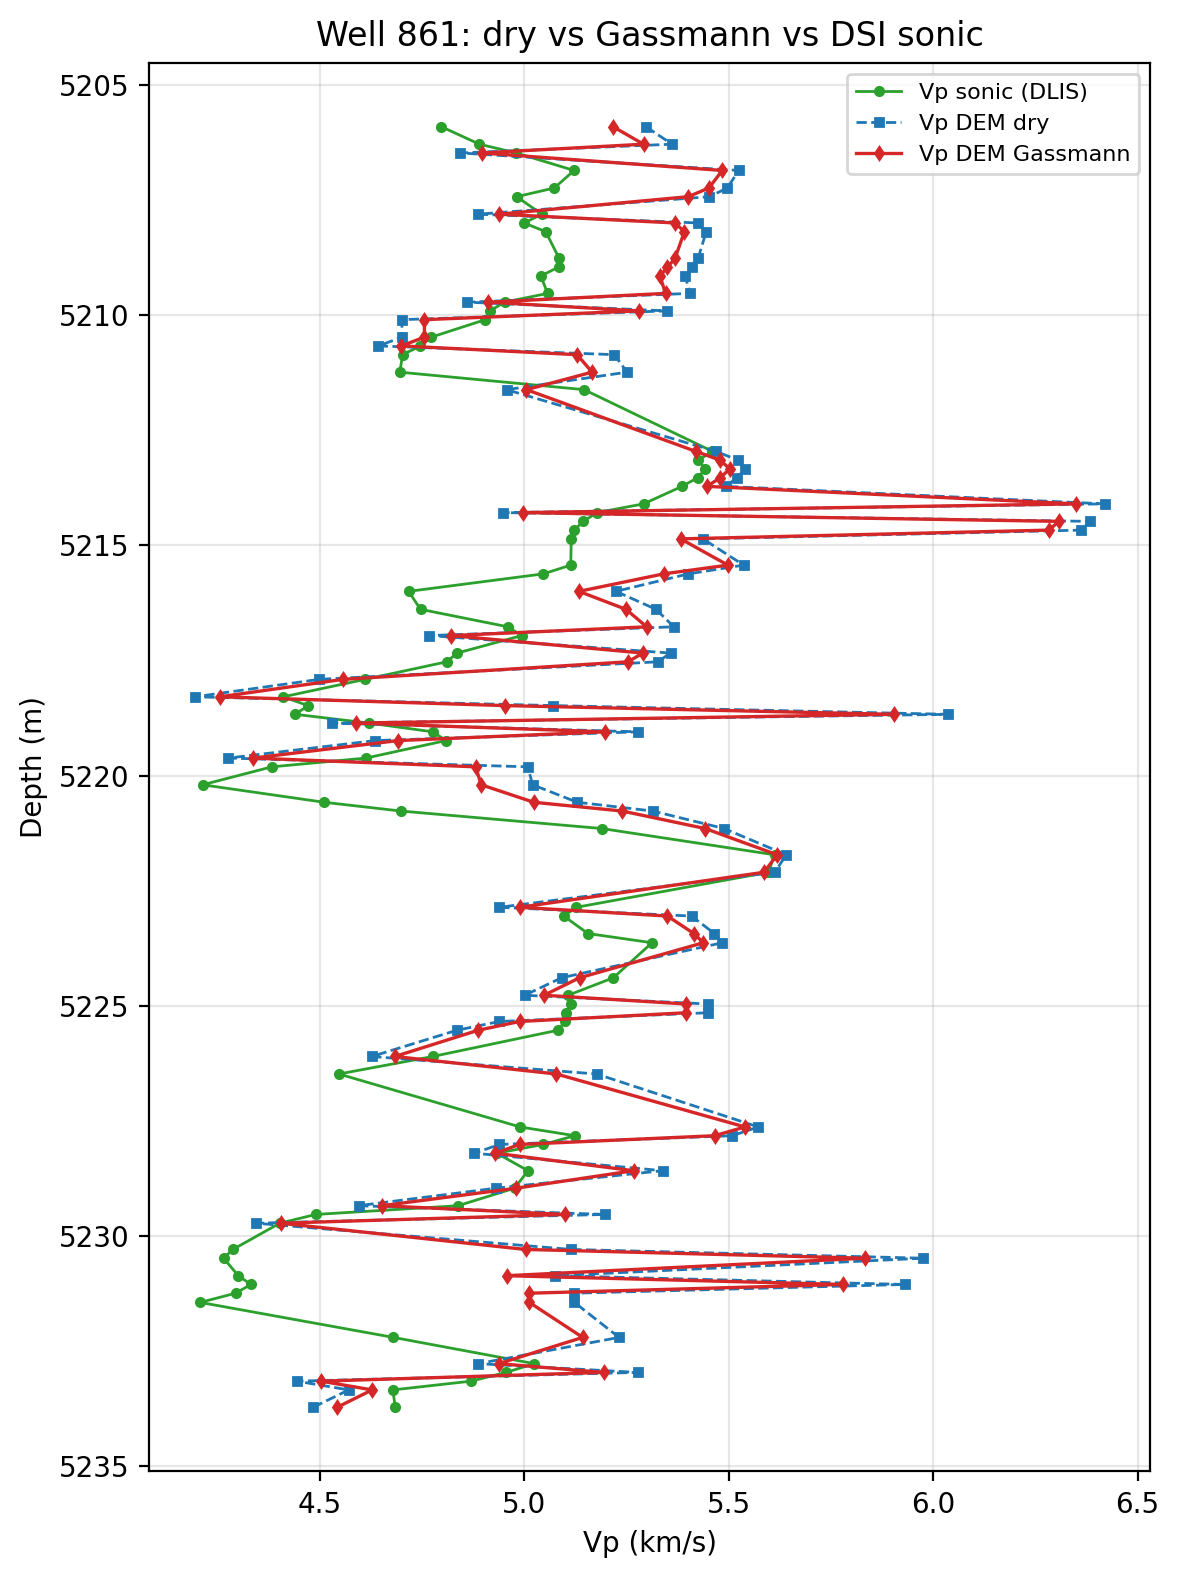
\includegraphics[width=0.78\linewidth]{figures/fig2_vp_dry_gassmann_sonic_depth}
  \caption{Trilha de profundidade: \Vp{} sónico (verde), DEM seco (azul tracejado)
           e DEM com Gassmann (vermelho). A saturacao aproxima parcialmente o
           sónico, mas não elimina o viés sistemático.}
  \label{fig:gassmann_depth}
\end{figure}

A Tabela~\ref{tab:gassmann_compare} e a Figura~\ref{fig:gassmann_depth} indicam
que Gassmann com $K_f$ default explica apenas uma fração do viés
observado: o modelo permanece $\approx 0{,}27$~km/s mais rápido que o DSI em
média.
O efeito é pequeno pela própria física do problema: com porosidade média de
$\approx 11\%$ e arcabouço rígido, o ganho de $K_{\mathrm{sat}}$ é quase
compensado pelo aumento de densidade, e o saldo líquido em \Vp{} fica em
poucos centésimos de km/s.
Por HFU, a saturação melhora todas as unidades na mesma proporção
(8,0\% $\rightarrow$ 6,8\% na HFU~1; 3,3\% $\rightarrow$ 2,2\% na HFU~2;
13,6\% $\rightarrow$ 11,5\% na HFU~3; 30,4\% $\rightarrow$ 28,1\% na HFU~4),
ou seja, não corrige o problema estrutural da HFU~4.
Possíveis causas residuais incluem pressão efetiva distinta entre lab
(22,1~MPa) e \emph{in-situ}, litologia local não capturada pela segmentação
HFU (especialmente HFU~4) e ausência de PVT medido in situ para refinar $K_f$.
Vale notar que \VpVs{} piora levemente após Gassmann (erro médio absoluto de
0,073 para 0,084): a saturação afeta $K_{\mathrm{sat}}$ e deixa
$G_{\mathrm{dry}}$ intacto, de modo que ganhos em \Vp{} absoluto vêm ao custo
da razão elástica.

\subsection{Validação tripla (lab, \phiS{}, DSI)}

A Tabela~\ref{tab:validation_triple} sintetiza as três pernas de validação
adotadas nesta etapa: laboratório nos plugs, consistência de porosidade com
\phiS{} e confronto elástico com o sónico (seco e Gassmann).

\begin{table}[H]
  \centering
  \caption{Validação tripla da Etapa~2: o que cada perna testa e o
           patamar obtido (rodada junho de 2026).}
  \label{tab:validation_triple}
  \small
  \begin{tabular}{llcc}
    \toprule
    Perna & Pergunta & Métrica & Valor \\
    \midrule
    Laboratório (LOO) & Fecha \Vp{} a seco nos plugs? & MAPE (\%) & 14,8 \\
    Entrada (\phiND{} vs \phiS) & Porosidade confiável? & Pearson $r$ & 0,94 \\
    Saída DSI (seco) & Extrapola \Vp{} \emph{in-situ}? & Viés (km/s) & $+0{,}30$ \\
    Saída DSI (Gassmann) & Fluido reduz o viés? & Viés (km/s) & $+0{,}27$ \\
    \bottomrule
  \end{tabular}
\end{table}

A validação tripla mostra que a \emph{entrada} petrofísica está sólida
($r \approx 0{,}94$), a \emph{física} fecha o laboratório seco (LOO $\approx 15\%$)
e a \emph{saída} contra o DSI fica em patamar utilizável ($\approx 7\%$ após
Gassmann), porém com viés positivo persistente.
Como esse viés é sistemático e concentrado nas unidades com pouco suporte de
laboratório, ele é candidato natural a correção estatística---o que motiva a
Etapa~3 sobre resíduos, e não o abandono do DEM/SC.

\section{DEM multiescala com frações NMR/CMR (fase~2g)}
\label{sec:multiscale_nmr}

\subsection{Motivação e escopo}

O teste A/B da fase~2f (Seção~\ref{sec:multiscale_ab}) mostrou que medianas de
frações meso-macro e micro do microCT por HFU (dois a quatro plugs) não
superam o monoescala calibrado no modo \emph{forward} relevante ao perfil.
A hipótese da fase~2g é que o particionamento macro/micro do CMR
(Schlumberger), disponível \textbf{continuamente} ao longo do poço, substitua
essas medianas frágeis sem reabrir a calibração elástica por HFU.

Executamos um experimento \textbf{aditivo} que \textbf{não altera} os parâmetros
calibrados na Etapa~2e ($\alpha$, $K_{\mathrm{scale}}$, $G_{\mathrm{scale}}$)
nem reajusta modulos ao sónico.
Comparamos:
\begin{itemize}
  \item \textbf{M1} --- monoescala Gassmann com $\phi = \phiND{}$ (baseline do
        perfil após fase~2b);
  \item \textbf{M3} --- DEM sequencial meso-macro + micro com frações NMR
        ponto a ponto, seguido de Gassmann com o mesmo fluido default
        ($K_f \approx 2{,}2$~GPa, $S_w = 1$).
\end{itemize}
As razões de aspecto $\alpha_{\mathrm{meso}}$ e $\alpha_{\mathrm{micro}}$
permanecem fixas por HFU (medianas da fase~2f); apenas as frações volumétricas
passam a variar com a profundidade via CMR.
Essa restrição é deliberada: o experimento isola o efeito das frações NMR
sem reabrir a calibração de geometria (Figura~\ref{fig:nmr_knobs}).
Em termos operacionais, o M3 libera o ``botão'' das frações contínuas e
mantém travados $\phi=\phiND{}$, a matriz calibrada e o AR por HFU.
Como a razão de aspecto controla grande parte da ``moleza'' elástica no
DEM, esperar ganho grande apenas com CMFF/BFV seria otimista demais---o
resultado empírico confirma essa leitura.

\begin{figure}[H]
  \centering
  \begin{tikzpicture}[
    knob/.style={
      draw, thick, rounded corners=2pt, align=center,
      text width=2.55cm, inner sep=4pt, font=\footnotesize,
      minimum height=1.15cm
    },
  ]
    \node[font=\normalsize\bfseries] at (0,1.7) {M1 monoescala};
    \node[knob, fill=blue!8, draw=blue!50!black] at (-3.9,0.55) {$\phi=\phiND{}$};
    \node[knob, fill=blue!8, draw=blue!50!black] at (-1.3,0.55) {$\alpha$ efetivo\\por HFU};
    \node[knob, fill=blue!8, draw=blue!50!black] at (1.3,0.55) {matriz $K,G$};
    \node[knob, fill=blue!8, draw=blue!50!black] at (3.9,0.55) {Gassmann};

    \node[font=\normalsize\bfseries] at (0,-0.85) {M3 NMR multiescala};
    \node[knob, fill=blue!8, draw=blue!50!black] at (-3.9,-2.0) {$\phi=\phiND{}$\\{\scriptsize (igual)}};
    \node[knob, fill=yellow!25, draw=orange!70!black] at (-1.3,-2.0) {%
      \textbf{frações NMR}\\{\scriptsize CMFF/BFV}
    };
    \node[knob, fill=gray!15, draw=gray] at (1.3,-2.0) {%
      AR meso/micro\\{\scriptsize \textbf{fixo} por HFU}
    };
    \node[knob, fill=blue!8, draw=blue!50!black] at (3.9,-2.0) {matriz +\\Gassmann};
  \end{tikzpicture}
  \caption{Desenho do experimento da fase~2g: apenas as frações
           macro/micro passam a variar com a profundidade via CMR; a
           razão de aspecto permanece constante por HFU. A ausência de ganho
           de MAPE é coerente com esse desenho.}
  \label{fig:nmr_knobs}
\end{figure}

No DEM sequencial, as inclusões são aplicadas em ordem de incremento de
porosidade $\phi_{\mathrm{inc}}=f_{\mathrm{pore}}\times\phi_{\mathrm{total}}$
\textbf{decrescente} (maior volume primeiro), alinhada à referência
Equinor/Berryman do projeto.
Essa ordem é por contribuição volumétrica, não por ``maior impacto
elástico'': poros achatados (baixo $\alpha$) podem amolecer mais por
unidade de volume do que poros arredondados.

\subsection{Extração e merge do CMR}

Extraímos curvas do arquivo \texttt{3-brsa-861-sps\_8\_cmr\_ecs.dlis}
(\texttt{logical\_file[0]}, frame 75B) com \texttt{extract\_861\_cmr.py}:
TDEP, CMRP\_3MS, CMFF e BFV.
A calibração de profundidade usou correlação com o GR do perfil integrado
(\texttt{861\_integrated\_logs\_enriched.xlsx}), obtendo escala
$\mathrm{TDEP}/393{,}7$ e correlação GR $\approx 0{,}99$.
Após recorte ao intervalo 5205,9--5233,7~m, restaram 152 amostras CMR
(CMRP\_3MS médio $\approx 0{,}11$, faixa 0,03--0,23).

O merge com o perfil Gassmann de 87 linhas (\texttt{merge\_asof}, tolerância
0,5~m) casou \textbf{87/87} profundidades.
As frações de porosidade usadas no DEM sequencial são:
\begin{equation}
  \label{eq:nmr_fractions}
  f_{\mathrm{macro}}^{\mathrm{NMR}} = \frac{\mathrm{CMFF}}{\mathrm{CMFF}+\mathrm{BFV}},
  \qquad
  f_{\mathrm{micro}}^{\mathrm{NMR}} = \frac{\mathrm{BFV}}{\mathrm{CMFF}+\mathrm{BFV}}.
\end{equation}
A porosidade total de entrada permanece $\phiND{}$; CMRP\_3MS entra apenas
no controle de qualidade e na validação cruzada com CT, não substitui
$\phiND{}$ no forward (teste auxiliar com $\phi = \mathrm{CMRP\_3MS}$ no M1
piorou o MAPE: 8,4\% contra 7,3\% com \phiND{}).

\subsection{Validação CMR versus microCT}

Nos dez plugs com microCT, comparamos $f_{\mathrm{macro}}^{\mathrm{CT}}$ e
$f_{\mathrm{micro}}^{\mathrm{CT}}$ (segmentação GeoDict) com as frações NMR
interpoladas na profundidade do plug.
A concordância é \textbf{fraca}: Pearson $r \approx -0{,}30$ tanto para macro
quanto para micro; o erro absoluto médio de $f_{\mathrm{macro}}$ é
$\approx 0{,}25$ em escala 0--1.
Isso indica que o particionamento CMR (CMFF/BFV) e o do microCT
(meso-macroporos/microporos) \textbf{não são equivalentes} termo a termo,
embora ambos capturem heterogeneidade de porosidade.
A Figura~\ref{fig:multiscale_nmr_ct} resume o contraste nos dez plugs.

\begin{figure}[H]
  \centering
  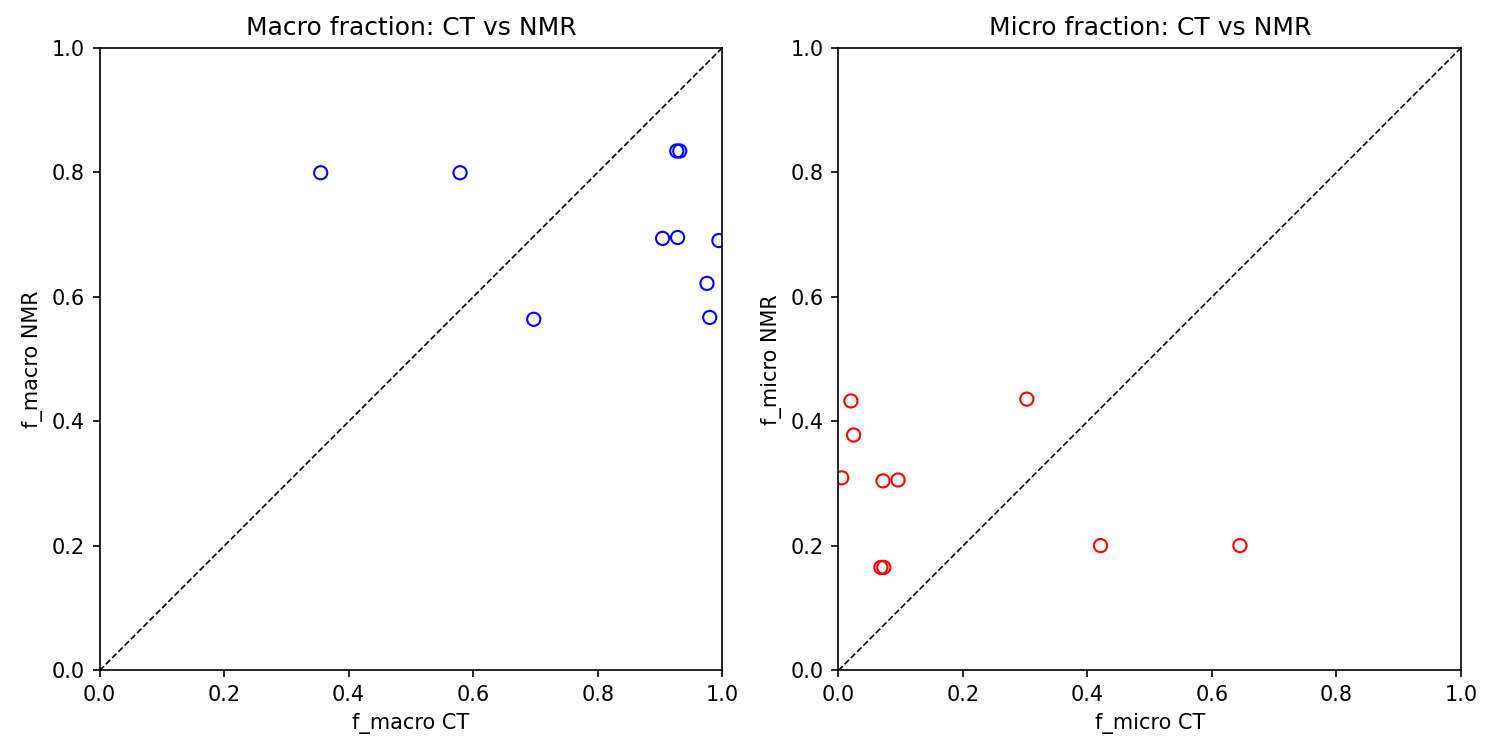
\includegraphics[width=0.55\linewidth]{figures/fig2_multiscale_nmr_ct_vs_nmr}
  \caption{Frações macro CT versus NMR nos dez plugs com microCT.
           A correlacao e fraca ($r \approx -0{,}30$), alertando para nao
           tratar CMFF/BFV como proxy direto da segmentacao CT.}
  \label{fig:multiscale_nmr_ct}
\end{figure}

\subsection{Resultados M1 versus M3 no perfil}

A Tabela~\ref{tab:multiscale_nmr} resume as métricas contra o sónico DSI nas
87 linhas com CMR casado.
O M3 praticamente elimina o viés, de $+0{,}27$ (M1) para $+0{,}04$~km/s, e
reduz marginalmente o RMSE (0,48 para 0,47~km/s), mas \textbf{piora} o MAPE
de 7,3\% para 8,5\%---$\Delta \approx -1{,}2$~p.p., no sentido oposto ao
limiar pre-registrado de $+2$~p.p.
A leitura é que o M3 troca acerto sistemático por dispersão: centra melhor a
distribuição do erro, porém espalha mais os pontos individuais.
A correlação de Pearson com o sónico é semelhante nos dois modelos
($r \approx 0{,}42$ e $0{,}45$), indicando que o particionamento NMR não
reorganiza o padrão espacial do erro de forma material.

\begin{table}[H]
  \centering
  \caption{DEM multiescala NMR versus monoescala Gassmann no perfil
           (87 linhas, junho de 2026). Parametros elásticos fixos por HFU;
           frações NMR ponto a ponto.}
  \label{tab:multiscale_nmr}
  \small
  \begin{tabular}{lcccc}
    \toprule
    Modelo & MAPE (\%) & RMSE (km/s) & Viés (km/s) & Pearson $r$ \\
    \midrule
    M1 monoescala Gassmann & 7,3 & 0,48 & $+0{,}27$ & $+0{,}42$ \\
    M3 multiescala NMR + Gassmann & 8,5 & 0,47 & $+0{,}04$ & $+0{,}45$ \\
    \bottomrule
  \end{tabular}
\end{table}

\textbf{Conclusão:} manter o produto monoescala Gassmann no perfil de 87
linhas; as frações CMR documentam variabilidade local de porosidade, mas não
justificam substituir o encadeamento M1 com o limiar adotado.
A Figura~\ref{fig:multiscale_decision} resume o critério pré-registrado
aplicado às fases~2f e~2g: só se promove multiescala se o ganho de MAPE
frente ao M1 for de pelo menos 2~p.p.\ de forma consistente.
No poço~861, nenhum dos dois experimentos atingiu esse limiar.
O experimento completo, scripts e \texttt{metrics.json} estão em
\texttt{dem\_sc\_runs/multiscale\_nmr/}; o planejamento em
\texttt{planning/etapa2g\_dem\_multiscale\_nmr\_poco861.md}.

\begin{figure}[H]
  \centering
  \begin{tikzpicture}[
    box/.style={
      draw=blue!50!black, thick, rounded corners=2pt, fill=blue!8,
      align=center, text width=3.2cm, inner sep=5pt, font=\small
    },
    q/.style={
      draw=orange!70!black, thick, rounded corners=2pt, fill=orange!10,
      align=center, text width=4.2cm, inner sep=5pt, font=\small
    },
    no/.style={
      draw=red!60!black, thick, rounded corners=2pt, fill=red!5,
      align=center, text width=4.0cm, inner sep=5pt, font=\small
    },
    arr/.style={-{Stealth[length=2.4mm]}, thick, blue!50!black},
  ]
    \node[box] (m1) at (0,1.6) {M1 monoescala\\(baseline)};
    \node[box] (m2) at (4.2,1.6) {M2b CT forward\\(fase~2f)};
    \node[box] (m3) at (8.4,1.6) {M3 NMR\\(fase~2g)};
    \node[q] (q) at (4.2,0.05) {Ganho MAPE $\geq 2$~p.p.\ vs M1?};
    \node[no] (n) at (4.2,-1.55) {%
      Não $\rightarrow$ \textbf{manter monoescala}\\
      {\footnotesize (caso do poço~861)}
    };
    \draw[arr] (m1) -- (q);
    \draw[arr] (m2) -- (q);
    \draw[arr] (m3) -- (q);
    \draw[arr] (q) -- (n);
  \end{tikzpicture}
  \caption{Critério de decisão das fases~2f e~2g: o produto de 87 linhas
           só migra para multiescala se o ganho frente ao monoescala
           atingir o limiar pré-registrado de 2~p.p.}
  \label{fig:multiscale_decision}
\end{figure}

A Figura~\ref{fig:multiscale_nmr_panel} contrasta M1 e M3 no plano 1:1 e ao
longo da profundidade; a Figura~\ref{fig:multiscale_nmr_fractions} mostra as
frações NMR no intervalo do poço.

\begin{figure}[H]
  \centering
  \begin{subfigure}[t]{0.48\linewidth}
    \centering
    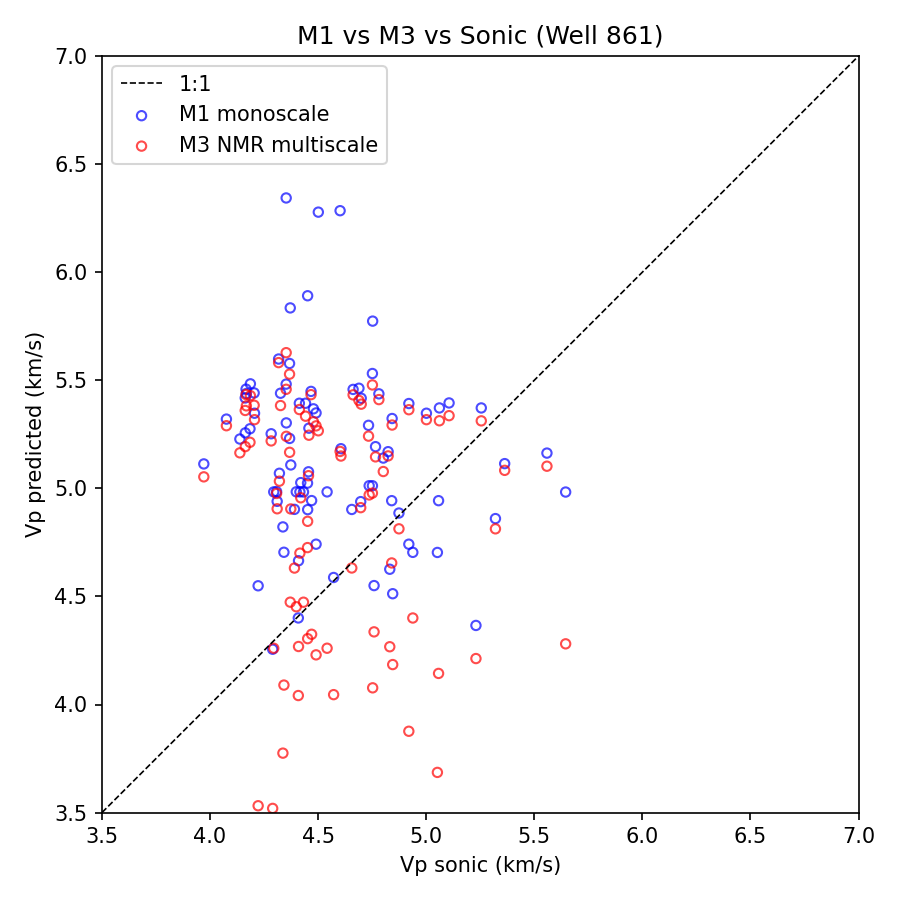
\includegraphics[width=\linewidth]{figures/fig2_multiscale_nmr_crossplot_vp}
    \caption{M1 versus M3 no plano 1:1 (sónico no eixo $y$).}
    \label{fig:multiscale_nmr_crossplot}
  \end{subfigure}
  \hfill
  \begin{subfigure}[t]{0.48\linewidth}
    \centering
    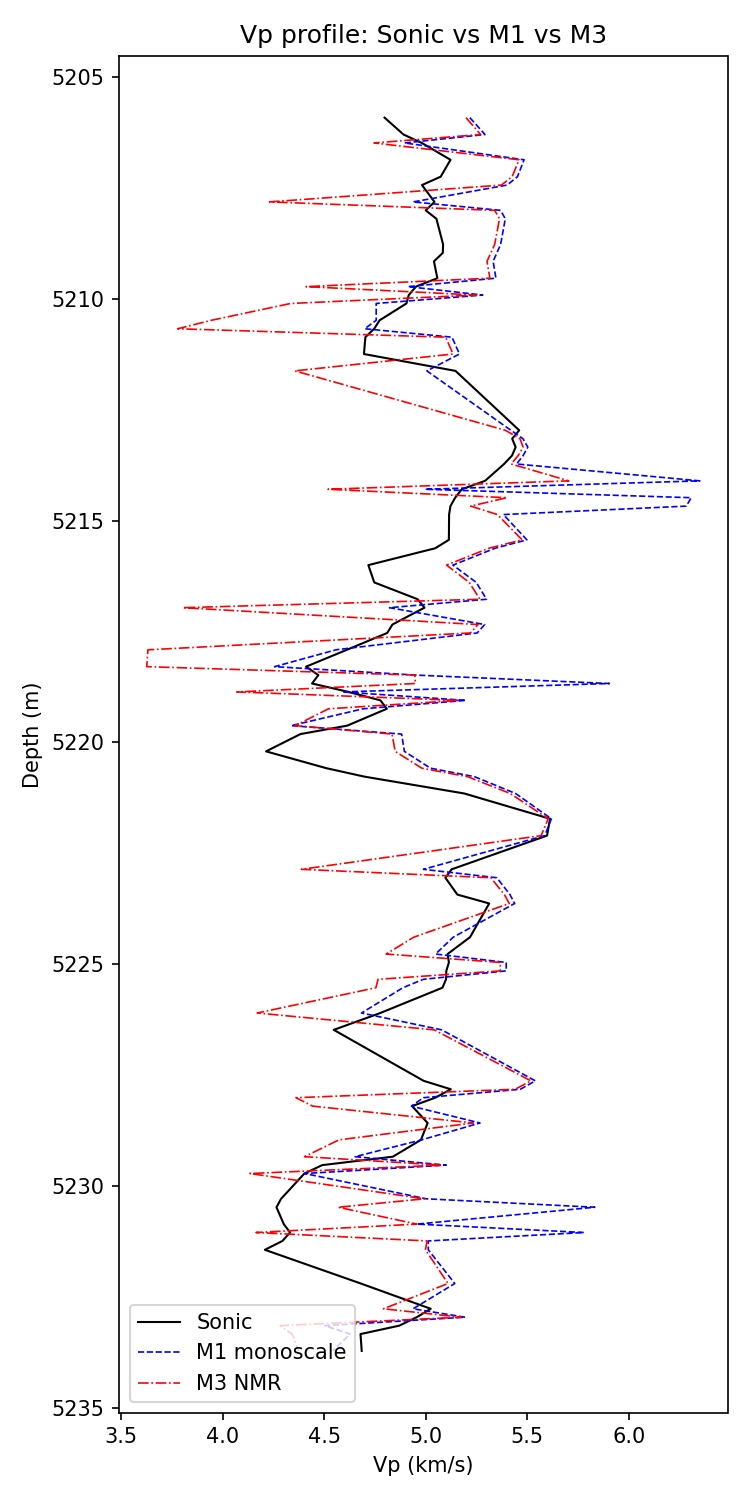
\includegraphics[width=\linewidth]{figures/fig2_multiscale_nmr_profile_vp}
    \caption{Trilha de \Vp{}: sónico, M1 e M3.}
    \label{fig:multiscale_nmr_profile}
  \end{subfigure}
  \caption{DEM multiescala NMR (fase~2g): ganho marginal frente ao monoescala
           Gassmann no perfil de 87 linhas.}
  \label{fig:multiscale_nmr_panel}
\end{figure}

\begin{figure}[H]
  \centering
  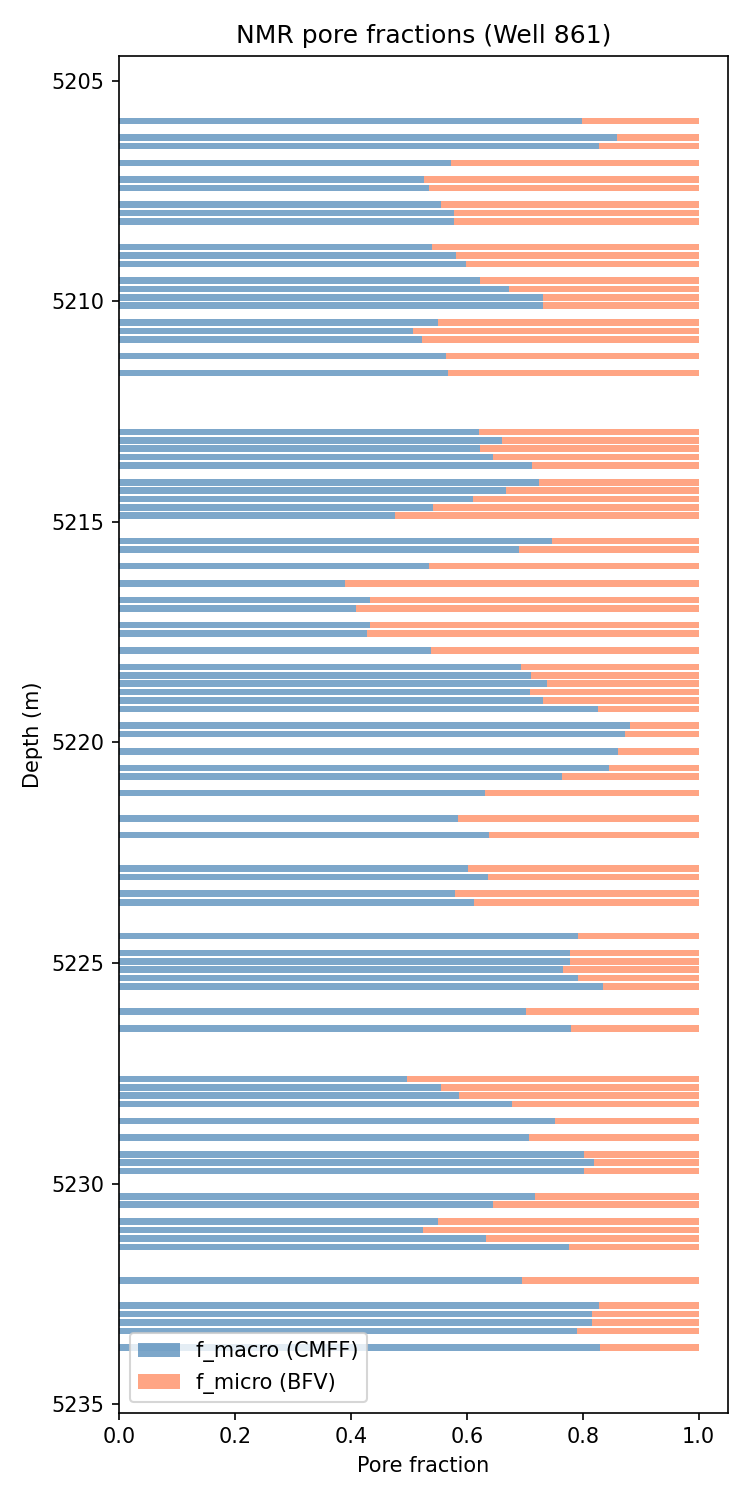
\includegraphics[width=0.78\linewidth]{figures/fig2_multiscale_nmr_fractions}
  \caption{Frações macro (CMFF) e micro (BFV) do CMR ao longo da profundidade
           no intervalo 5205,9--5233,7~m.}
  \label{fig:multiscale_nmr_fractions}
\end{figure}

A fraqueza residual do M3---$\alpha_{\mathrm{micro}}$ ainda fixo por HFU com
apenas dois a quatro plugs de suporte---limita o ganho mesmo quando as frações
variam ponto a ponto; combinar NMR com inversão local de $\alpha_{\mathrm{micro}}$
fica fora do escopo desta rodada.

\section{Discussão}
\label{sec:discussao}

Esta seção sintetiza os achados da
Tabela~\ref{tab:validation_summary} sob três eixos: viabilidade da
modelagem física, limites das condições experimentais e encaminhamento
para saturação e aprendizado sobre resíduos.

\subsection{O modelo físico funciona, mas exige calibração por HFU}

A prova de conceito (Seção~\ref{sec:poc}) mostrou implementação
estável; a validação sem calibração (Seção~\ref{sec:lab})
mostrou que parâmetros crus do microCT não bastam.
A calibração inversa por HFU reduz o MAPE de $\approx 26\%$ para
$\approx 9\%$ (\emph{in-sample}) e para $\approx 15\%$ no LOO---patamar
honesto para dez plugs do poço~861.
Isso confirma a estratégia definida na Etapa~1: segmentar por HFU de
laboratório e usar CT na física, não no ML de perfil.
A calibração não deve ser apresentada como generalizável sem ressalva:
é \textbf{ajuste local por HFU} sustentado por dez plugs neste poço.

\subsection{Escopo da validação: intra-poço}

Todas as métricas elásticas contra o DSI referem-se ao \textbf{mesmo poço}
(87/87 profundidades casadas).
Demonstram consistência local no intervalo do campo Lapa e indicam \emph{potencial} de
generalização, mas \textbf{não substituem} validação interpoços.
A extrapolação do perfil calibrado faz sentido como aplicação local;
transferência a outros poços carbonáticos exige novos plugs e recalibração.

\subsection{\Vp{} absoluto versus \VpVs{}}

\VpVs{} concorda com o sónico dentro de um erro médio absoluto de
$\approx 0{,}07$ (cerca de 4\% da razão média), enquanto \Vp{} isolado
carrega viés de $+0{,}30$~km/s.
Em termos práticos, o produto desta etapa é mais confiável para
discriminar unidades de fluxo e tendências litológicas do que para
estimar módulos absolutos prontos para inversão sísmica sem correção
de fluido.
Reforça essa leitura o fato de \VpVs{} degradar levemente após Gassmann,
enquanto \Vp{} melhora: as duas grandezas respondem a mecanismos diferentes e
não devem ser otimizadas pelo mesmo critério.

\subsection{Por que o sónico diverge do laboratório calibrado}

O LOO apresenta viés praticamente nulo contra plugs secos; o perfil sónico
apresenta viés positivo sistemático.
A diferença não contradiz o pipeline---aponta para \textbf{condições
físicas distintas}: laboratório (seco, 22,1~MPa, escala de plug) versus
sónico (saturado, \emph{in-situ}, escala de investigação maior).
A fase~2b com Gassmann e $K_f$ default reduziu o viés de $+0{,}30$ para
$+0{,}27$~km/s (Tabela~\ref{tab:gassmann_compare}), confirmando que parte do
desvio seca/saturada é real---mas não suficiente para alinhar o perfil ao
DSI.
Etapa~3 deve focar resíduos locais (HFU~3, HFU~4) e não substituir a cadeia
física por ML direto.

\subsection{HFU~4 e HFU~3: zonas de cautela}
\label{sec:hfu_cautela}

A HFU~4 não possui plug de calibração e apresenta MAPE $\approx 30\%$
contra o sónico; não deve ser usada em entregas interpretativas sem novos
dados.
A HFU~3 tem apenas dois plugs: o LOO é instável e o erro de perfil
($\approx 14\%$) é aceitável, mas não robusto.
A HFU~2 é o \emph{benchmark} interno do poço nesta etapa, com
$\approx 3\%$ contra o sónico.

Os dois extremos da gradação 3\%, 8\%, 14\%, 30\% são consistentes com o
suporte experimental: a HFU~2, com quatro plugs, é a melhor, e a HFU~4, sem
nenhum, é a pior.
A ordenação completa, porém, \textbf{não} é explicada pelo número de plugs:
HFU~1 e HFU~2 dispõem de quatro plugs cada e diferem por um fator de 2,4 no
MAPE de perfil.
O que separa essas duas unidades é a saturação de $\alpha$.
Na Tabela~\ref{tab:hfu_params}, a HFU~1 e a HFU~3 têm $\alpha$ calibrado no
teto do intervalo (0,950), enquanto a HFU~2 fica no interior (0,182); no
laboratório pós-calibração as duas unidades saturadas ficam em 11,0\% e
10,2\% de MAPE contra 6,8\% da unidade não saturada.
Com o número de plugs controlado em quatro, portanto, o discriminante
observado é a saturação do parâmetro---um limite de \emph{parametrização} do
DEM, e não escassez amostral.

A leitura defensável é que os erros maiores se concentram nas unidades com
menor ou nenhum suporte experimental, mas que esta etapa \textbf{não separa}
as contribuições de amostragem, litologia e limitação de formulação.
Com quatro HFUs, contagens de plugs confundidas (quatro, quatro, dois e zero)
e dois casos de $\alpha$ no teto, não há graus de liberdade para atribuir o
erro a uma única causa.
Afirmar que o gargalo é exclusivamente amostral seria mais forte do que os
dados sustentam, e a saturação de $\alpha$ é evidência direta em contrário.

\subsection{Multiescala sequencial: sem ganho para o perfil}

O teste A/B da Seção~\ref{sec:multiscale_ab} mostra que decompor porosidade
em meso-macro e micro (DEM sequencial, referência Equinor) \textbf{nao}
substitui o monoescala calibrado no cenario de extrapolacao ao perfil quando
as fracoes vem de medianas CT por HFU.
O modo \emph{oracle}---ajustar $\alpha_{\mathrm{micro}}$ plug a plug ao
laboratório---reduz o MAPE para $\approx 3\%$, mas isso e diagnostico de
ajustabilidade, nao previsao.
O modo \emph{forward} (medianas HFU, sem inversao no plug avaliado)
praticamente replica o MAPE \emph{in-sample} do M1 (8,7\% contra 9,1\%); o LOO
melhora $\approx 2{,}9$~p.p., sem confirmacao \emph{in-sample}.
A fase~2g (Seção~\ref{sec:multiscale_nmr}) repete o exercicio com fracoes NMR
ponto a ponto no perfil de 87 linhas: o M3 nao melhora o MAPE frente ao M1
Gassmann---piora $\approx 1{,}2$~p.p.---e a validacao CMR versus CT nos dez
plugs mostra correlacao fraca ($r \approx -0{,}30$).
Esse resultado e coerente com o desenho do experimento
(Figura~\ref{fig:nmr_knobs}): as fracoes variam com a profundidade, mas a
razao de aspecto do micro---que controla grande parte da resposta
elastica---permanece fixa por HFU.
Mantemos $\alpha$ efetivo por HFU no produto de 87 linhas; as fracoes
multiescala do CT e do CMR ficam arquivadas para estudos futuros (p.ex.\ poco~1045
ou novos plugs).

\subsection{Relação com a Etapa~1 e caminho para a Etapa~3}

As decisões da Etapa~1 permanecem válidas: \phiND{} como entrada, HFU de
laboratório, microCT na física, validação espacialmente honesta.
O aprendizado de máquina direto perfil $\rightarrow$ \Vp{} continua
descartado.
A Etapa~3 deve atuar sobre \emph{resíduos} (\Vp{} observado menos \Vp{}
físico), após a fase~2b documentada na Seção~\ref{sec:gassmann}.

\section{Conclusões e recomendações}
\label{sec:conclusoes}

\begin{enumerate}
  \item \textbf{Viabilidade:} a modelagem DEM/SC calibrada por HFU é
        \emph{consistente} com o sónico de perfil no poço~861
        ($\approx 9\%$ a seco, $\approx 7\%$ após Gassmann) e
        \emph{parcialmente consistente} com o laboratório sob a métrica mais
        severa (LOO $\approx 15\%$ nos dez plugs).
        Trata-se de \textbf{prova de conceito física local}, não de
        validação interpoços.
  \item \textbf{Uso por HFU:} confiar na HFU~2 ($\approx 3\%$) e na HFU~1
        ($\approx 8\%$); usar HFU~3 ($\approx 14\%$) com ressalvas
        documentadas; evitar HFU~4 ($\approx 30\%$) até obter plugs ou
        calibração independente.
        Os maiores erros concentram-se nas unidades com menor ou nenhum
        suporte experimental, o que torna a aquisição de plugs na HFU~4 a
        intervenção de maior retorno esperado; o número de plugs,
        isoladamente, não explica toda a variação
        (Seção~\ref{sec:hfu_cautela}).
  \item \textbf{Entrada de porosidade:} manter \phiND{} (correlação
        $r \approx 0{,}94$ com \phiS{}) como default; RF de \philab{} permanece
        alternativa documentada da Etapa~1.
  \item \textbf{Multiescala (fase~2f):} DEM sequencial meso-macro + micro
        nao supera o monoescala calibrado no modo \emph{forward} relevante
        ao perfil (MAPE \emph{in-sample} 8,7\% contra 9,1\%, dentro do ruído
        de dez plugs); manter $\alpha$ efetivo por HFU
        (Seção~\ref{sec:multiscale_ab}).
  \item \textbf{Multiescala NMR (fase~2g):} fracoes CMR ponto a ponto no
        perfil reduzem o viés de $+0{,}27$ para $+0{,}04$~km/s, mas elevam o
        MAPE de 7,3\% para 8,5\%; o critério pre-registrado exige ganho de
        2~p.p.\ em MAPE, logo manter monoescala Gassmann
        (Seção~\ref{sec:multiscale_nmr}).
  \item \textbf{Fase~2b (Gassmann):} com $K_f \approx 2{,}2$~GPa e $S_w=1$, o
        MAPE contra o DSI cai de 8,7\% para 7,3\% e o viés de $+0{,}30$ para
        $+0{,}27$~km/s---melhora consistente, porém sem eliminar o desvio
        sistemático.
  \item \textbf{Etapa~3:} considerar aprendizado sobre resíduos da física
        (HFU~3 e HFU~4 prioritárias), não substituição da cadeia
        DEM/SC por ML de perfil.
        Como o resíduo é dominado por uma componente sistemática por unidade
        de fluxo, o alvo natural é um corretor de baixa complexidade, com
        validação por blocos de profundidade para não superestimar o ganho.
\end{enumerate}

\section*{Disponibilidade dos dados e reprodutibilidade}

A ingestão da planilha ROCKPHYS, a extração do perfil sónico DSI, os
pipelines de meio efetivo DEM/SC, calibração por HFU, teste A/B multiescala,
extração CMR/NMR, substituição de fluido Gassmann e validações laboratorial,
LOO e sónicas foram
implementados de forma automatizada e reprodutível no repositório do projeto
\emph{methods\_comparison}.
Os conjuntos processados, métricas numéricas e figuras podem ser obtidos
mediante acesso ao repositório ou solicitação aos autores, no mesmo
espírito do relatorio da Etapa~1.
Os numeros citados neste documento correspondem à rodada de producao de
junho de 2026, registrada nos manifestos e arquivos de métricas exportados
por cada etapa do pipeline.

\appendix

\section{Modelagem numérica de meio efetivo}
\label{app:dem_core}

Este apêndice formaliza a cadeia elástica usada na Etapa~2 do poço~861:
da matriz carbonática aos módulos a seco (Differential Effective Medium, DEM,
e esquema auto-consistente, SC), da densidade às velocidades de fase e,
na fase~2b, à substituição de fluido de Gassmann.
O objetivo é permitir que o leitor reproduza o raciocínio físico \textbf{sem}
consultar o código-fonte: cada equação abaixo corresponde a um estágio do
pipeline numérico automatizado do repositório.

\subsection{Objetivo e encadeamento}

Na Etapa~1, a porosidade de perfil (\phiND{}) mostrou-se a propriedade mais
acessível ao longo das 87 linhas; a velocidade elástica, porém, depende de
\emph{como} os poros enfraquecem a matriz---geometria, mineralogia e rigidez
do arcabouco.
Os modelos de meio efetivo respondem a essa pergunta ao traduzir
$(\phi,\,\alpha,\,K_m,\,G_m)$ em módulos efetivos a seco
$K_{\mathrm{dry}}$ e $G_{\mathrm{dry}}$, onde $\alpha$ é a razão de aspecto
dos poros e $(K_m,G_m)$ descrevem a matriz mineral.

Adotamos o DEM de Berryman como trilha principal e o SC como controle de
consistência interna: nos dez plugs com microCT, as duas teorias diferem em
menos de 1\% em \Vp{} antes da calibração, sinal de que o gargalo petrofísico
está nos parâmetros de entrada, não na escolha entre formalismos.
A Tabela~\ref{tab:app_chain} resume o encadeamento completo; as subseções
seguintes detalham cada etapa.

\begin{table}[H]
  \centering
  \caption{Encadeamento físico da modelagem numérica de meio efetivo
           (poço~861, rodada junho de 2026).}
  \label{tab:app_chain}
  \small
  \begin{tabular}{p{2.8cm}p{3.2cm}p{3.2cm}p{4.5cm}}
    \toprule
    Etapa & Entrada & Saída & Papel petrofísico \\
    \midrule
    Mistura VRH & Frações calcita/dolomita & $K_m$, $G_m$, $\rho_m$ & Matriz mineral \\
    DEM / SC & $\phi$, $\alpha$, $K_m$, $G_m$ & $K_{\mathrm{dry}}$, $G_{\mathrm{dry}}$ & Arcabouco a seco \\
    Densidade & $\phi$, $\rho_m$ (e fluido na 2b) & $\rho_{\mathrm{eff}}$ & Massa específica \\
    Gassmann (2b) & $K_{\mathrm{dry}}$, $K_0$, $K_f$, $\phi$ & $K_{\mathrm{sat}}$ & Saturação isotrópa \\
    Velocidades & $K$, $G$, $\rho_{\mathrm{eff}}$ & \Vp, \Vs, \VpVs & Comparação lab/DSI \\
    \bottomrule
  \end{tabular}
\end{table}

Na Tabela~\ref{tab:app_chain}, a coluna ``Etapa'' segue a ordem em que o
pipeline aplica as transformações: primeiro a matriz, depois o arcabouco poroso,
então a massa e, quando pertinente, o fluido de poro, fechando em
velocidades observáveis em laboratório ou perfil.

\subsection{Matriz mineral e unidades de trabalho}

Todas as grandezas elásticas internas usam gigapascal (GPa); densidades em
g/cm$^3$; velocidades exportadas em m/s e km/s.
A conversão para unidades SI na velocidade segue
$1\,\mathrm{GPa} = 10^9\,\mathrm{Pa}$ e
$1\,\mathrm{g/cm^3} = 1000\,\mathrm{kg/m^3}$.

A Tabela~\ref{tab:app_minerals} lista os end-members adotados para o intervalo
campo Lapa (carbonatos calcíticos/dolomíticos), com propriedades de referência
da literatura de física de rochas.
A Tabela~\ref{tab:app_plug_mineral} traz, plug a plug, as frações
\textit{volume corrected} do microCT, as frações normalizadas $f_1$, $f_2$ e
os modulos $K_m$, $G_m$, $\rho_m$ resultantes da mistura VRH \emph{antes} da
calibração inversa.
A Tabela~\ref{tab:app_plug_lab} reúne porosidade de laboratório, $\alpha_{\mathrm{CT}}$
e velocidades de referência ROCKPHYS (22,1~MPa, eixo~$Z$).
A Tabela~\ref{tab:app_hfu_matrix} condensa a extrapolação por HFU; a
Tabela~\ref{tab:app_pvt} fixa o fluido de Gassmann; a
Tabela~\ref{tab:app_numerical} registra limites numéricos.

Dadas frações volumétricas normalizadas $f_1$ (calcita) e $f_2$
(dolomita), cada propriedade $M$ (bulk $K$, cisalhamento $G$ ou densidade
$\rho$) é estimada pela média de Hill sobre os limites de Voigt e Reuss:
\begin{align}
  M_{\mathrm{V}} &= \sum_{j} f_j\, M_j,
  &
  M_{\mathrm{R}} &= \left(\sum_{j} \frac{f_j}{M_j}\right)^{-1},
  &
  M_{\mathrm{VRH}} &= \frac{M_{\mathrm{V}} + M_{\mathrm{R}}}{2}.
  \label{eq:vrh}
\end{align}
Na Equacao~\eqref{eq:vrh}, $M_{\mathrm{V}}$ e o limite superior (isostresse)
e $M_{\mathrm{R}}$ o limite inferior (isodistensão); a média de Hill e o
ponto médio usual em rochas poliminerais.
Os modulos da matriz antes da calibração são
$K_m = M_{\mathrm{VRH}}(K_{\mathrm{calcita}},K_{\mathrm{dolomita}})$ e
analogamente para $G_m$ e $\rho_m$, a partir das frações corrigidas de
cada plug ou da extrapolação por unidade hidrodinamica de fluxo (HFU).

\begin{table}[H]
  \centering
  \caption{Propriedades elásticas e densidade dos end-members mineralógicos
           (defaults campo Lapa, literatura de carbonatos).}
  \label{tab:app_minerals}
  \begin{tabular}{lcccc}
    \toprule
    Mineral & $K$ (GPa) & $G$ (GPa) & $\rho$ (g/cm$^3$) & Papel no modelo \\
    \midrule
    Calcita   & 77 & 32 & 2,71 & Solido~1 (segmentacao CT) \\
    Dolomita  & 95 & 45 & 2,87 & Solido~2 (segmentacao CT) \\
    \bottomrule
  \end{tabular}
\end{table}

\begin{table}[H]
  \centering
  \caption{Frações mineralógicas corrigidas (microCT) e matriz VRH por plug
           (antes da calibração inversa). Solido~1/Solido~2 em \%; $f_1$, $f_2$
           normalizados entre os dois solidos.}
  \label{tab:app_plug_mineral}
  \scriptsize
  \setlength{\tabcolsep}{3pt}
  \begin{tabular}{lrrrrrrrrrr}
    \toprule
    Plug & Prof.\ (m) & HFU &
    S1 (\%) & S2 (\%) & $f_1$ & $f_2$ &
    $K_m$ & $G_m$ & $\rho_m$ \\
    \midrule
    F2829V & 5206,00 & 3 & 49,5 & 50,5 & 0,495 & 0,505 & 85,6 & 38,0 & 2,79 \\
    F2830H & 5206,05 & 3 & 88,4 &  5,3 & 0,943 & 0,057 & 77,9 & 32,6 & 2,72 \\
    F2852H & 5211,40 & 1 & 17,6 & 79,3 & 0,182 & 0,818 & 91,4 & 42,3 & 2,84 \\
    F2854H & 5212,05 & 2 & 93,8 &  2,3 & 0,976 & 0,024 & 77,4 & 32,3 & 2,71 \\
    F2859H & 5212,90 & 1 & 26,8 & 68,2 & 0,282 & 0,718 & 89,5 & 40,9 & 2,82 \\
    F2870H & 5215,55 & 1 & 95,3 &  4,2 & 0,958 & 0,042 & 77,7 & 32,5 & 2,72 \\
    F2880H & 5218,25 & 2 & 29,7 & 58,5 & 0,337 & 0,663 & 88,5 & 40,1 & 2,82 \\
    F2910H & 5225,70 & 2 & 13,6 & 74,4 & 0,155 & 0,845 & 91,9 & 42,7 & 2,84 \\
    F2911V & 5225,75 & 2 & 80,9 &  4,2 & 0,951 & 0,049 & 77,8 & 32,5 & 2,72 \\
    F2935H & 5232,25 & 1 & 74,8 &  7,2 & 0,912 & 0,088 & 78,4 & 33,0 & 2,72 \\
    \bottomrule
  \end{tabular}
\end{table}

\begin{table}[H]
  \centering
  \caption{Entradas elásticas e de laboratório por plug (dez amostras com
           microCT casadas a ROCKPHYS). $\phi_{\mathrm{lab}}$ em fração v/v;
           pressão de referência 22,1~MPa.}
  \label{tab:app_plug_lab}
  \scriptsize
  \setlength{\tabcolsep}{4pt}
  \begin{tabular}{lrrrrrrr}
    \toprule
    Plug & HFU & $\phi_{\mathrm{lab}}$ &
    $\alpha_{\mathrm{CT}}$ &
    \Vp{} lab (km/s) & \Vs{} lab (km/s) & \VpVs{} lab \\
    \midrule
    F2829V & 3 & 0,110 & 0,678 & 4,955 & 2,972 & 1,667 \\
    F2830H & 3 & 0,110 & 0,552 & 5,787 & 3,344 & 1,731 \\
    F2852H & 1 & 0,103 & 0,582 & 5,811 & 3,452 & 1,683 \\
    F2854H & 2 & 0,075 & 0,538 & 5,033 & 2,978 & 1,690 \\
    F2859H & 1 & 0,090 & 0,537 & 5,127 & 3,016 & 1,700 \\
    F2870H & 1 & 0,155 & 0,551 & 5,941 & 3,563 & 1,667 \\
    F2880H & 2 & 0,181 & 0,560 & 4,610 & 2,814 & 1,638 \\
    F2910H & 2 & 0,131 & 0,569 & 4,963 & 2,957 & 1,678 \\
    F2911V & 2 & 0,131 & 0,547 & 3,818 & 2,241 & 1,704 \\
    F2935H & 1 & 0,115 & 0,557 & 4,483 & 2,612 & 1,716 \\
    \bottomrule
  \end{tabular}
\end{table}

\begin{table}[H]
  \centering
  \caption{Matriz e geometria por HFU: mediana CT, valores calibrados contra
           laboratório e escalas $s_K$, $s_G$. A HFU~4 usa média das matrizes
           CT das HFU~2 e~3 (\emph{fallback}, sem escala laboratorial).}
  \label{tab:app_hfu_matrix}
  \small
  \setlength{\tabcolsep}{3pt}
  \begin{tabular}{crrrrrrrrr}
    \toprule
    HFU & $n$ &
    $\alpha_{\mathrm{CT}}$ & $\alpha_{\mathrm{calib}}$ &
    $K_m^{\mathrm{CT}}$ & $G_m^{\mathrm{CT}}$ &
    $K_m^{\mathrm{calib}}$ & $G_m^{\mathrm{calib}}$ &
  $\rho_m$ & $s_{K,G}$ \\
    \midrule
    1 & 4 & 0,554 & 0,950 & 84,0 & 36,9 & 58,6 & 25,7 & 2,774 & 0,697 \\
    2 & 4 & 0,554 & 0,182 & 83,2 & 36,3 & 59,0 & 25,8 & 2,766 & 0,709 \\
    3 & 2 & 0,615 & 0,950 & 81,8 & 35,3 & 59,0 & 25,5 & 2,754 & 0,721 \\
    4 & 0 & --    & 0,566 & 82,5 & 35,8 & 82,5 & 35,8 & 2,760 & 1,000 \\
    \bottomrule
  \end{tabular}
\end{table}

\begin{table}[H]
  \centering
  \caption{Parâmetros de fluido para Gassmann (fase~2b, default campo Lapa).}
  \label{tab:app_pvt}
  \begin{tabular}{lc}
    \toprule
    Grandeza & Valor adotado \\
    \midrule
    Fluido & Salmoura de formação (default) \\
    $K_f$ (GPa) & 2,2 \\
    $\rho_f$ (g/cm$^3$) & 1,03 \\
    $S_w$ & 1,0 (saturação total) \\
    Pressão de referência (MPa) & 22,1 \\
    Temperatura de referência ($^\circ$C) & 60 \\
    \bottomrule
  \end{tabular}
\end{table}

\begin{table}[H]
  \centering
  \caption{Limites e constantes numéricas do esquema DEM/SC (poço~861).}
  \label{tab:app_numerical}
  \begin{tabular}{lc}
    \toprule
    Parametro & Valor \\
    \midrule
    Porosidade $\phi$ (entrada DEM) & \philab{} nos plugs; \phiND{} no perfil \\
    Limite inferior de $\phi$ & $10^{-4}$ \\
    Limite superior de $\phi$ & 0,95 \\
    $\alpha$ na calibração & $[0{,}15,\,0{,}95]$ \\
    Iterações SC & 80 \\
    Inclusões de poro & $K_i = G_i = 0$ (arcabouço seco) \\
    \bottomrule
  \end{tabular}
\end{table}

A porosidade de entrada é limitada ao intervalo
$\phi \in [10^{-4},\,0{,}95]$ por estabilidade numérica: na integração do DEM,
a variável auxiliar $y$ não pode aproximar-se de 1, onde o denominador
$(1-y)$ da Equacao~\eqref{eq:dem_k} se anula.
Na calibração (Apêndice~\ref{app:dem_calib}), fatores multiplicativos $s_K$ e
$s_G$ podem reduzir ou aumentar $K_m$ e $G_m$ de forma uniforme dentro de
limites fisicamente plausíveis.

\subsection{Geometria dos poros: fatores $P$ e $Q$}

Para inclusões esferoidais com razão de aspecto $\alpha$ (oblatos com
$\alpha < 1$, prolados com $\alpha > 1$), Berryman (1980) define fatores de
concentração de deformação $P$ e $Q$ que dependem dos módulos da fase
hospedeira $(K,G)$, da inclusão $(K_i,G_i)$ e de $\alpha$.
Esses fatores entram nas equações diferenciais do DEM e quantificam o quanto
uma inclusao ``mole'' (poro vazio) enfraquece o meio efetivo para dada
geometria.

No caso esferico ($\alpha = 1$), as expressões fechadas sao
\begin{align}
  P &= \frac{K + \frac{4}{3}G}{K_i + \frac{4}{3}G},
  &
  \xi &= \frac{G}{6}\,\frac{9K + 8G}{K + 2G},
  &
  Q &= \frac{G + \xi}{G_i + \xi}.
  \label{eq:pq_sphere}
\end{align}
Para esferoides gerais, definem-se funções auxiliares $\theta(\alpha)$ e
$F(\alpha)$ a partir de integrais geométricas (oblatos e prolados), e $P$ e $Q$
sao obtidos dos invariantes de Eshelby agregados $T_{iijj}$ e $T_{ijij}$:
\begin{equation}
  P = \frac{T_{iijj}}{3},
  \qquad
  Q = \frac{T_{ijij} - T_{iijj}}{5}.
  \label{eq:pq_general}
\end{equation}
Em todo o pipeline do poço~861, os poros sao tratados como inclusões
\emph{secas}, ou seja, $K_i = G_i = 0$: o fluido entra apenas na etapa de
Gassmann (Subsecao~\ref{app:gassmann}).

\subsection{Modelo DEM de Berryman}

\paragraph{Ideia fisica.}
O DEM imagina a rocha como matriz sólida em $y=0$ e adiciona, de forma
infinitesimal, uma fração $dy$ de inclusões vazias até atingir a porosidade
alvo $\phi$.
A cada passo, os módulos efetivos $(K_{\mathrm{eff}}, G_{\mathrm{eff}})$ sao
atualizados; no início, $K_{\mathrm{eff}}(0)=K_m$ e $G_{\mathrm{eff}}(0)=G_m$.

\paragraph{Equações e integração.}
Berryman (1992) escreve o sistema acoplado em $y \in [0,\phi]$:
\begin{align}
  (1-y)\,\frac{dK_{\mathrm{eff}}}{dy} &= (K_i - K_{\mathrm{eff}})\,P^*,
  \label{eq:dem_k} \\
  (1-y)\,\frac{dG_{\mathrm{eff}}}{dy} &= (G_i - G_{\mathrm{eff}})\,Q^*,
  \label{eq:dem_g}
\end{align}
onde $P^*$ é e $Q^*$ sao recalculados a cada passo com os módulos efetivos
instantaneos $(K_{\mathrm{eff}}, G_{\mathrm{eff}})$---a não linearidade do
problema reside precisamente nessa atualização.
O sistema é resolvido numericamente sobre uma malha uniforme de passo
$\Delta y \approx 0{,}005$, construída de modo que o ultimo no coincida
\emph{exatamente} com $y = \phi$;
$(K_{\mathrm{dry}}, G_{\mathrm{dry}})$ correspondem a esse ultimo ponto da
trajetoria.
A ancoragem do no final é essencial: uma malha que ultrapasse $\phi$ congela
os modulos em intervalos curtos de porosidade enquanto a densidade continua
variando, o que inverteria localmente a relação \Vp{}--$\phi$ e introduziria
artefato de serrilhado no perfil.

Um teste de sensibilidade ao passo de integração, documentado na
Seção~\ref{sec:crosscheck_rockphypy} e na
Figura~\ref{fig:dem_rockphypy_crosscheck}, mostra variação de 2,7\%
em $K_{\mathrm{dry}}$ para $\Delta y \in [0{,}001,\,0{,}02]$ no plug F2854H.
O confronto com a biblioteca aberta RockPhysicsPy (v0.0.2) confirma que os
fatores $P$ e $Q$ locais seguem Berryman na ordem correta $(K, G)$, enquanto a
rotina diferencial \emph{publicada na biblioteca} invoca \emph{PQ} com bulk e
cisalhamento efetivos trocados---provável erro de implementação que
explica divergência média de cerca de 30\% em $K_{\mathrm{dry}}$ nos dez
plugs (detalhes na Seção~\ref{sec:crosscheck_rockphypy}).

\subsection{Esquema auto-consistente}

O esquema auto-consistente (SC) busca módulos $(K_{\mathrm{eff}}, G_{\mathrm{eff}})$
nos quais matriz e inclusão ``veem'' o mesmo meio homogeneizado.
Utilizamos a variante iterativa para inclusões secas, com razão de Poisson
efetiva
\begin{equation}
  \nu_{\mathrm{eff}} = \frac{3K_{\mathrm{eff}} - 2G_{\mathrm{eff}}}
                              {2(3K_{\mathrm{eff}} + G_{\mathrm{eff}})}
  \label{eq:nu_sc}
\end{equation}
e atualizações de $K_{\mathrm{eff}}$ e $G_{\mathrm{eff}}$ a cada iteração até
convergência prática (80 ciclos).
A saída $(K_{\mathrm{dry}}^{\mathrm{SC}}, G_{\mathrm{dry}}^{\mathrm{SC}})$
serve como controle: quando DEM e SC divergem pouco, reforca-se que a
incerteza dominante está na calibração de $\alpha$ e da matriz, não no
formalismo escolhido.

\subsection{Densidade e velocidades de fase}
\label{app:vel}

Para rocha seca, a densidade do arcabouco é
\begin{equation}
  \rho_{\mathrm{dry}} = (1-\phi)\,\rho_m.
  \label{eq:rho_dry}
\end{equation}
Com saturação $S_w$ e fluido de densidade $\rho_f$ na fase~2b:
\begin{equation}
  \rho_{\mathrm{sat}} = (1-\phi)\,\rho_m + \phi\,S_w\,\rho_f.
  \label{eq:rho_sat}
\end{equation}
Dados $K$ e $G$ em GPa e $\rho$ em g/cm$^3$, as velocidades de fase seguem
\begin{equation}
  V_p = \sqrt{\frac{K + \frac{4}{3}G}{\rho}},
  \qquad
  V_s = \sqrt{\frac{G}{\rho}},
  \label{eq:vp_vs_app}
\end{equation}
com conversão para SI antes da raiz quadrada.
A Equacao~\eqref{eq:vp_vs_app} e equivalente à~\eqref{eq:velocidades} do
corpo do texto, tomando $\rho_{\mathrm{eff}}$ como $\rho_{\mathrm{dry}}$ ou
$\rho_{\mathrm{sat}}$ conforme o estagio.
A razão \VpVs{} e derivada como grandeza adimensional para comparação com
laboratório e perfil sônico.

\subsection{Substituição de fluido de Gassmann}
\label{app:gassmann}

Após o arcabouco seco, a saturação isotrópa segue a forma padrao de Mavko
\emph{et al.}:
\begin{equation}
  K_{\mathrm{sat}} = K_{\mathrm{dry}}
  + \frac{\left(1 - \dfrac{K_{\mathrm{dry}}}{K_0}\right)^2}
         {\dfrac{\phi}{K_f} + \dfrac{1-\phi}{K_0}
          - \dfrac{K_{\mathrm{dry}}}{K_0^2}},
  \qquad
  G_{\mathrm{sat}} = G_{\mathrm{dry}}.
  \label{eq:gassmann}
\end{equation}
Na Equacao~\eqref{eq:gassmann}, $K_0$ é o bulk da matriz mineral
(pós-calibracao), $K_f$ o bulk do fluido de poro (default de formacao,
$\approx 2{,}2$~GPa na fase~2b) e $\phi$ a porosidade total.
O cisalhamento não muda: a saturação afeta principalmente \Vp{} via
$K_{\mathrm{sat}}$ e $\rho_{\mathrm{sat}}$, enquanto \Vs{} responde sobretudo
a $G_{\mathrm{dry}}$.

\section{Calibração inversa por unidade de fluxo}
\label{app:dem_calib}

Este apêndice descreve como ajustamos, \emph{separadamente para cada HFU com
plugs de laboratório}, os parâmetros petrofísicos que alimentam o DEM da
Secao~\ref{app:dem_core}, de modo a reduzir o erro de \Vp{} frente às
medidas ROCKPHYS (eixo~$Z$, 22,1~MPa, condição seca).

\subsection{Motivação e dados por plug}

A razão de aspecto mediana do microCT por HFU, usada sem ajuste, produz
erro percentual medio absoluto (MAPE) de cerca de 26\% contra o laboratório
(Seção~\ref{sec:lab}).
A calibração \textbf{não altera} a porosidade medida em laboratorio nem cria
amostras artificiais: apenas encontra $(\alpha, s_K, s_G)$ que minimizam o
desvio elástico \emph{dado} o modelo DEM e a mineralogia de cada plug.

Cada plug de calibração agrega: identificador e HFU de laboratório;
$\phi_{\mathrm{lab}}$ e estimativa de $\alpha$ pelo microCT; frações
mineralógicas corrigidas (calcita/dolomita); e \Vp, \Vs{} e \VpVs{} medidos
no eixo~$Z$.

\subsection{Modelo direto e função objetivo}

Para parametros candidatos $(\alpha, s_K, s_G)$, a predição de \Vp{} no plug
$k$ escreve-se
\begin{equation}
  \widehat{V}_{p,k}^{\mathrm{DEM}}
  = \mathcal{F}\!\left(
      \phi_k,\,\alpha,\,s_K K_m^{(k)},\,s_G G_m^{(k)}
    \right),
  \label{eq:vp_forward}
\end{equation}
onde $\mathcal{F}$ denota a composição VRH $\rightarrow$ DEM
$\rightarrow$ \eqref{eq:rho_dry} $\rightarrow$ \eqref{eq:vp_vs_app} e
$(K_m^{(k)}, G_m^{(k)})$ vem da mistura mineral do plug $k$.

Para o conjunto de plugs $\mathcal{P}_h$ da HFU $h$, adotamos o erro
quadratico medio (RMSE) em \Vp{} como função custo:
\begin{equation}
  \mathrm{RMSE}_{V_p}(\theta)
  = \sqrt{\frac{1}{|\mathcal{P}_h|}
    \sum_{k \in \mathcal{P}_h}
    \left(\widehat{V}_{p,k}^{\mathrm{DEM}}(\theta) - V_{p,k}^{\mathrm{lab}}\right)^2},
  \label{eq:rmse_vp}
\end{equation}
com $\theta = (\alpha)$ ou $\theta = (\alpha, s)$ conforme o cenario.
O pipeline também reporta o MAPE para diagnostico:
\begin{equation}
  \mathrm{MAPE}_{V_p}
  = \frac{100}{|\mathcal{P}_h|}
    \sum_{k}
    \frac{\left|\widehat{V}_{p,k}^{\mathrm{DEM}} - V_{p,k}^{\mathrm{lab}}\right|}
         {V_{p,k}^{\mathrm{lab}}},
  \label{eq:mape_vp}
\end{equation}
mas a otimização minimiza \eqref{eq:rmse_vp}, não \eqref{eq:mape_vp}, para
penalizar de forma quadratica os outliers de velocidade.

\subsection{Cenarios de ajuste}

A Tabela~\ref{tab:app_calib_scenarios} resume os dois cenarios testados por
HFU; o pipeline retem automaticamente o de menor RMSE após calibração.

\begin{table}[H]
  \centering
  \caption{Cenarios de calibração inversa por HFU (dez plugs CT, ROCKPHYS).
           Limites numericos da rodada junho de 2026.}
  \label{tab:app_calib_scenarios}
  \begin{tabular}{lp{5.5cm}p{5.5cm}}
    \toprule
    Cenario & Parâmetros livres & Restrições \\
    \midrule
    Somente $\alpha$ &
    $\theta = \alpha$; matriz fixa ($s_K = s_G = 1$) &
    $\alpha \in [0{,}15,\,0{,}95]$ \\
    $\alpha$ + escala de matriz &
    $\theta = (\alpha, s)$; $K_m \leftarrow s K_m$, $G_m \leftarrow s G_m$ &
    $\alpha \in [0{,}15,\,0{,}95]$, $s \in [0{,}50,\,1{,}50]$ \\
    \bottomrule
  \end{tabular}
\end{table}

Na Tabela~\ref{tab:app_calib_scenarios}, o segundo cenario permite compensar
rigidez mineral sistematicamente superestimada quando o microCT sozinho não
fecha o laboratório.
A busca usa o algoritmo L-BFGS-B com limites de caixa; para cada HFU com
plugs disponíveis ($h=1,2,3$), os parâmetros escolhidos alimentam a
extrapolacao ao perfil de 87 linhas.
A HFU~4 não possui plug de calibração e recebe parametros de
\emph{fallback} (media das HFU~2 e~3), conforme discutido na
Seção~\ref{sec:protocolo}.

\subsection{Validação leave-one-plug-out}

O ajuste \emph{in-sample} reduz o MAPE para cerca de 9\%, mas superestima a
capacidade de generalização dentro da mesma HFU.
Por isso adotamos validação \emph{leave-one-plug-out} (LOO): para cada plug
$k$, recalibra-se $\theta_h^{-k}$ apenas com $\mathcal{P}_h \setminus \{k\}$ e
prevê-se $\widehat{V}_{p,k}^{\mathrm{LOO}}$ sem usar a velocidade daquele
plug no ajuste.
O MAPE LOO de cerca de 15\% (Tabela~\ref{tab:validation_summary}) e a métrica
\emph{honesta} citada no resumo executivo; deve ser distinguido do ajuste
direto nos dez plugs.

\subsection{Encadeamento calibração--perfil--Etapa~3}

Os parâmetros calibrados por HFU alimentam a extrapolacao ao perfil completo
(87 linhas com \phiND{} e HFU de laboratório), primeiro a seco e depois com
Gassmann na fase~2b.
Um teste A/B multiescala (\emph{forward}, sem nova regressao global) nao
justificou trocar o monoescala por inclusoes sequenciais no produto de perfil
(Seção~\ref{sec:multiscale_ab}); a extensao com fracoes NMR/CMR ponto a ponto
tambem nao atingiu o limiar de ganho adotado (Seção~\ref{sec:multiscale_nmr}).
As velocidades teóricas saturadas confrontam-se com o perfil sônico DSI; o
desvio residual local motiva a Etapa~3 (correção de aprendizado de máquina
sobre o resíduo, não substituição do DEM).

Em sintese, o Apêndice~\ref{app:dem_core} responde \emph{como a física
transforma} $(\phi,\alpha,K_m,G_m)$ em \Vp; o Apêndice~\ref{app:dem_calib}
responde \emph{como ajustamos} $(\alpha,s)$ para fechar o laboratorio por HFU
sem alterar $\phi$, mantendo rastreabilidade entre prova de conceito, perfil
e validação honesta.

\end{document}
